\chapter{層ごとの学習過程に着目した検証}
\section{はじめに}
Heckelらは,モデルの異なる部分が異なるエポックで学習とし,層ごとに学習率を変更することで二重降下が緩和することを示している\cite{Heckel}.本章では,\cref{fig:overview}を観察した条件において,層ごとの特徴学習過程に着目した複数の検証を行う.今後の実験の理解を助けるために,ResNet18の構造を説明する.Heらの論文のTable 1を\cref{tab:ResNet_arch}に示す.ResNet18は,大まかに,17層の畳み込み層と1層の全結合層から構成される.また最初の層を除いた畳み込み層は,4層ごとにブロックを構成している.以降では,1層目の畳み込み層をconv1,4つのブロックを浅い位置から,block1,block2,block3,block4と呼称する.

\newcommand{\blocka}[2]{\multirow{3}{*}{\(\left[\begin{array}{c}\text{3$\times$3, #1}\\[-.1em] \text{3$\times$3, #1} \end{array}\right]\)$\times$#2}
}
\newcommand{\blockb}[3]{\multirow{3}{*}{\(\left[\begin{array}{c}\text{1$\times$1, #2}\\[-.1em] \text{3$\times$3, #2}\\[-.1em] \text{1$\times$1, #1}\end{array}\right]\)$\times$#3}
}
\begin{table}[htb]
\caption{ResNet architecture (citing Tab. 1 of [10]).}
\vspace{-.5em}
\begin{center}
\resizebox{0.9\linewidth}{!}{
%\footnotesize
\begin{tabular}{c|c|c|c|c|c|c}
\hline
layer name & output size & 18-layer & 34-layer & 50-layer & 101-layer & 152-layer \\
\hline
conv1 & 112$\times$112 & \multicolumn{5}{c}{7$\times$7, 64, stride 2}\\
\hline
\multirow{4}{*}{conv2\_x} & \multirow{4}{*}{56$\times$56} & \multicolumn{5}{c}{3$\times$3 max pool, stride 2} \\\cline{3-7}
  &  & \blocka{64}{2}  & \blocka{64}{3} & \blockb{256}{64}{3} & \blockb{256}{64}{3} & \blockb{256}{64}{3}\\
  &  &  &  &  &  &\\
  &  &  &  &  &  &\\
\hline
\multirow{3}{*}{conv3\_x} &  \multirow{3}{*}{28$\times$28}  & \blocka{128}{2}  & \blocka{128}{4}  & \blockb{512}{128}{4}  & \blockb{512}{128}{4}  &
                              \blockb{512}{128}{8}\\
  &  &  &  &  &  & \\
  &  &  &  &  &  & \\
\hline
\multirow{3}{*}{conv4\_x} & \multirow{3}{*}{14$\times$14}  & \blocka{256}{2}  & \blocka{256}{6}  & \blockb{1024}{256}{6}  & \blockb{1024}{256}{23} & \blockb{1024}{256}{36}\\
  &  &  &  &  & \\
  &  &  &  &  & \\
\hline
\multirow{3}{*}{conv5\_x} & \multirow{3}{*}{7$\times$7}  & \blocka{512}{2}  & \blocka{512}{3}  & \blockb{2048}{512}{3}  & \blockb{2048}{512}{3}
& \blockb{2048}{512}{3}\\
  &  &  &  &  &  & \\
  &  &  &  &  &  & \\
\hline
& 1$\times$1  & \multicolumn{5}{c}{average pool, 1000-d fc, softmax} \\
\hline
\multicolumn{2}{c|}{FLOPs} & 1.8$\times10^9$  & 3.6$\times10^9$  & 3.8$\times10^9$  & 7.6$\times10^9$  & 11.3$\times10^9$ \\
\hline
\end{tabular}
}
\end{center}
\vspace{-.5em}
\label{tab:ResNet_arch}
\vspace{-.5em}
\end{table}

\section{階層ごとの偏重度}
本研究では,形状・テクスチャ偏重度をモデルが持つ最終畳み込み層が出力する特徴マップから算出している.しかし,\cref{sec:形状・テクスチャ偏重度の定量化}の方法を使用して,異なる層からも形状・テクスチャへの偏重度が計算可能である.そのため,今まで使用していた17層(=block4の最後の畳み込み層)に対して,各blockの最後の畳み込み層(5層,9層,13層)で形状・テクスチャへの偏重度を算出し,最後の畳み込み層から算出した形状・テクスチャ偏重度の推移と比較した.

結果を\cref{fig:layer_ab}に示す.17層においては形状・テクスチャ偏重度が特異な推移をしているのに対して,5層,9層,13層における形状・テクスチャへの偏重度の推移は基本的に一定で推移している.このことから,深い層のみで見られる特性があると考えられる.また,この特性を理解することで,二重降下に対してのより深い理解への糸口となる可能性がある.
\begin{figure}[h]
\centering
\begin{minipage}[b]{.48\linewidth}
    \centering
    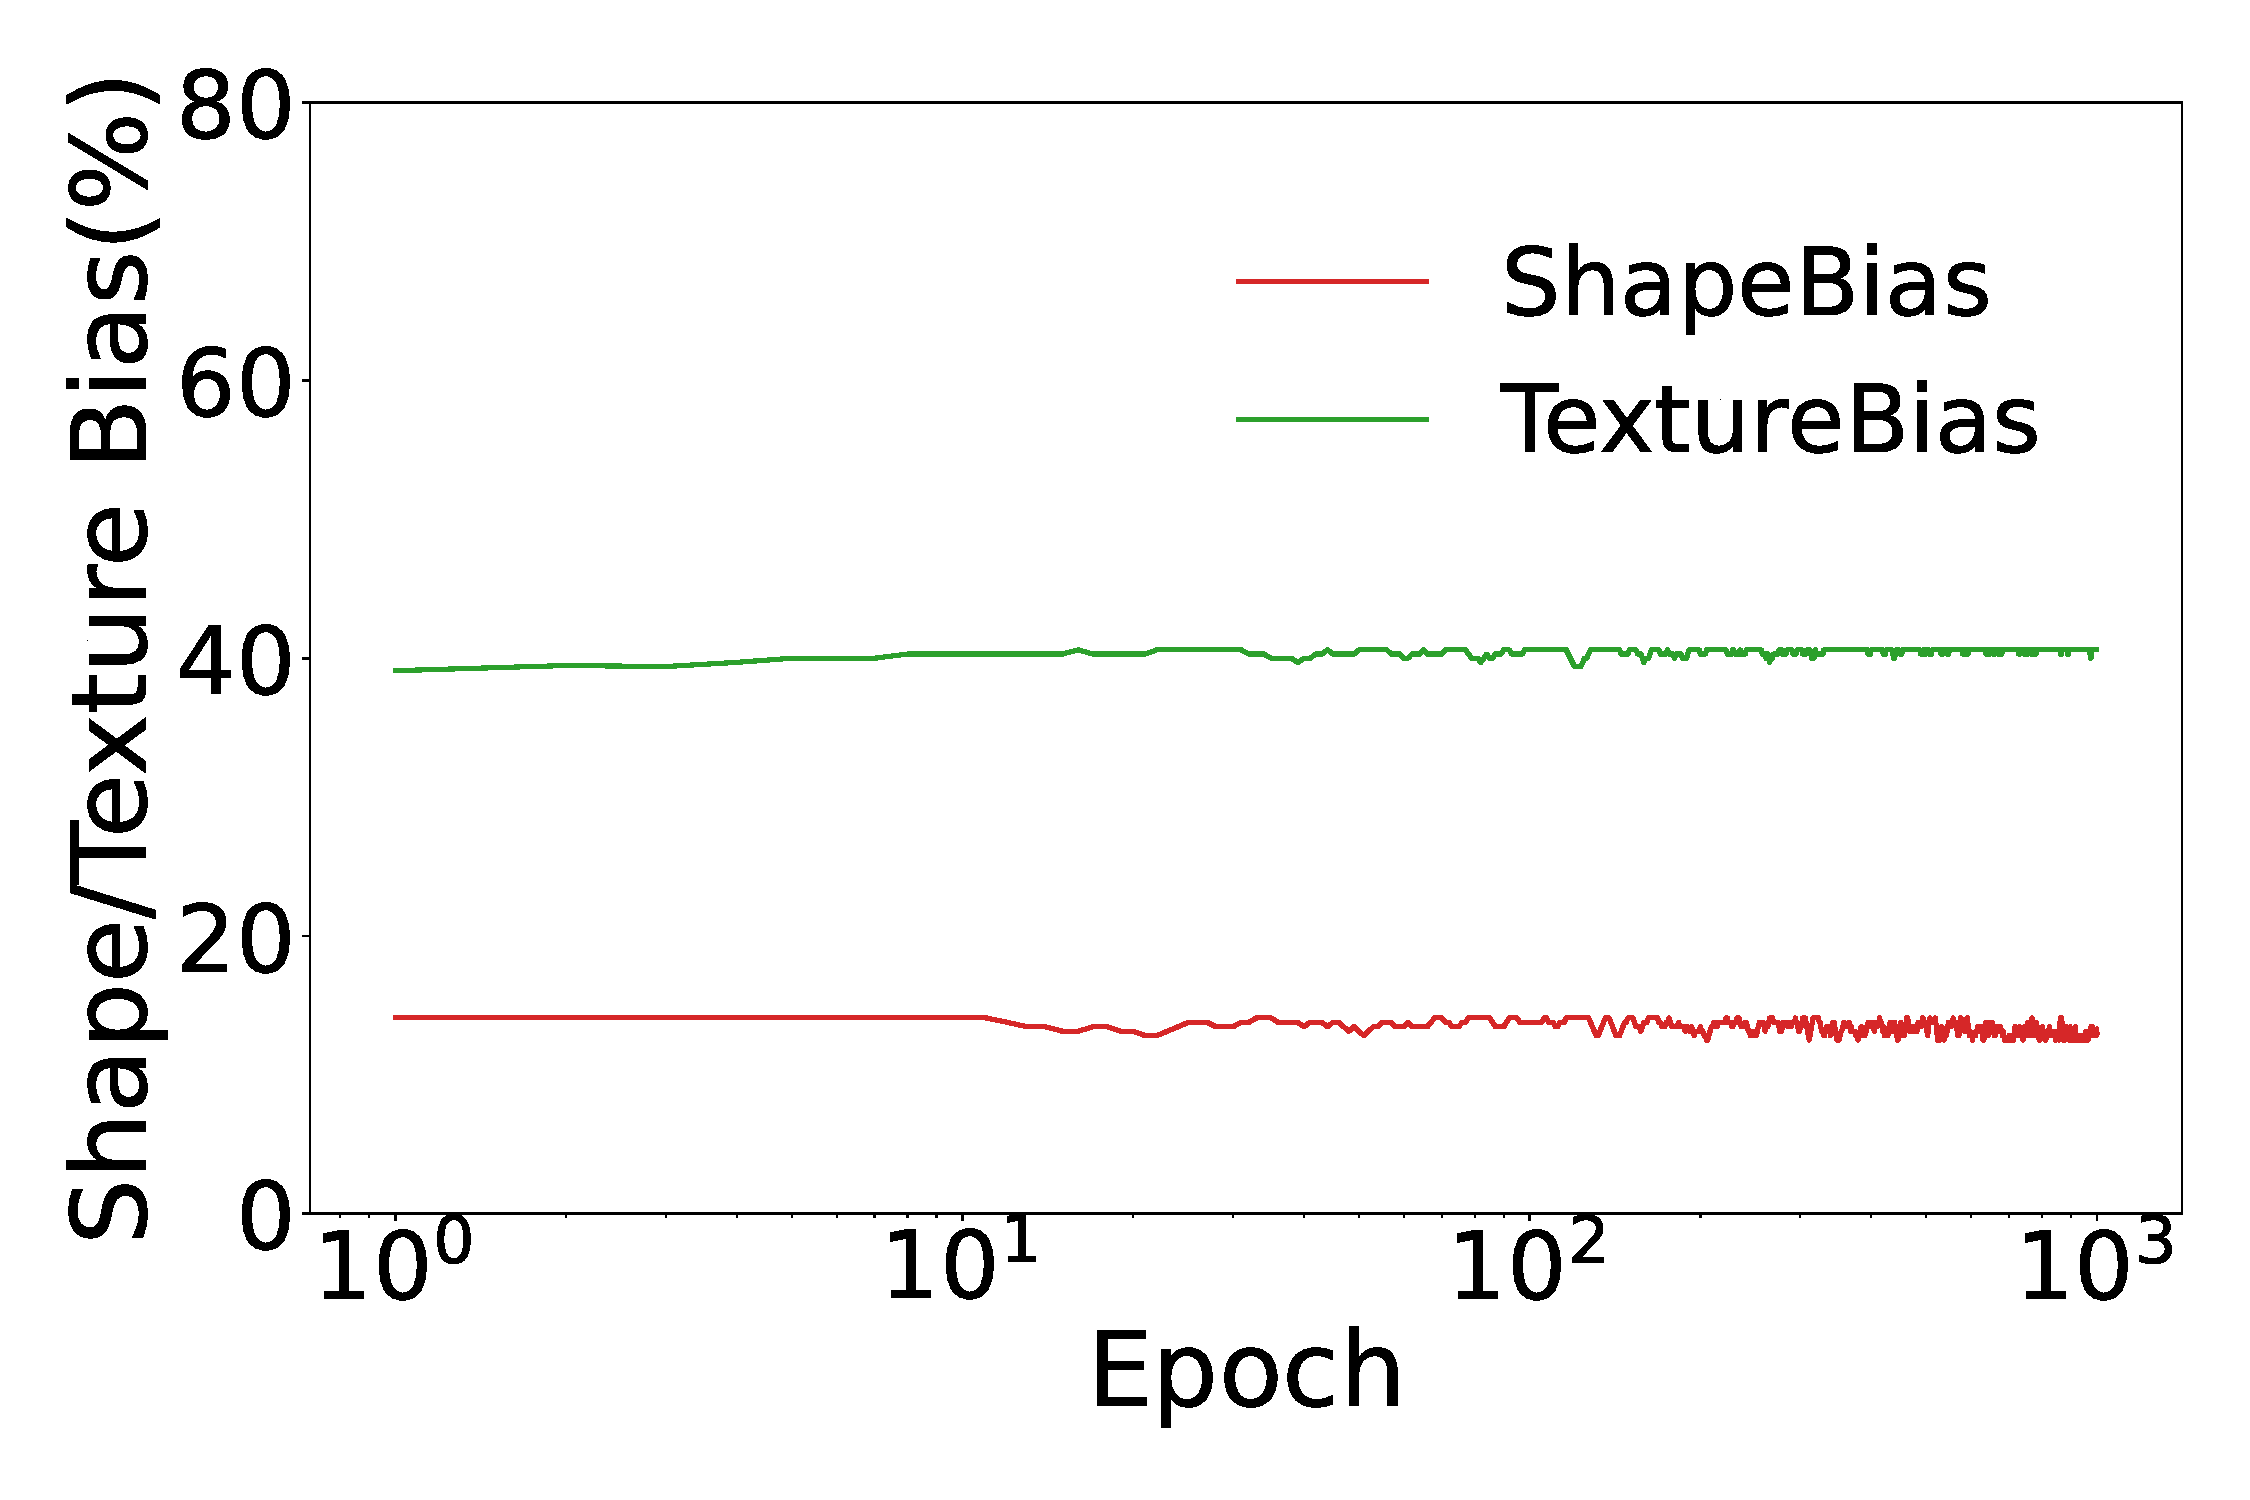
\includegraphics[width=1\linewidth]{bias_fig/IN_ResNet18/layer5.pdf}
    \subcaption{5th layer}% \caption{Figure caption}
  \end{minipage}
\begin{minipage}[b]{.48\linewidth}
    \centering
    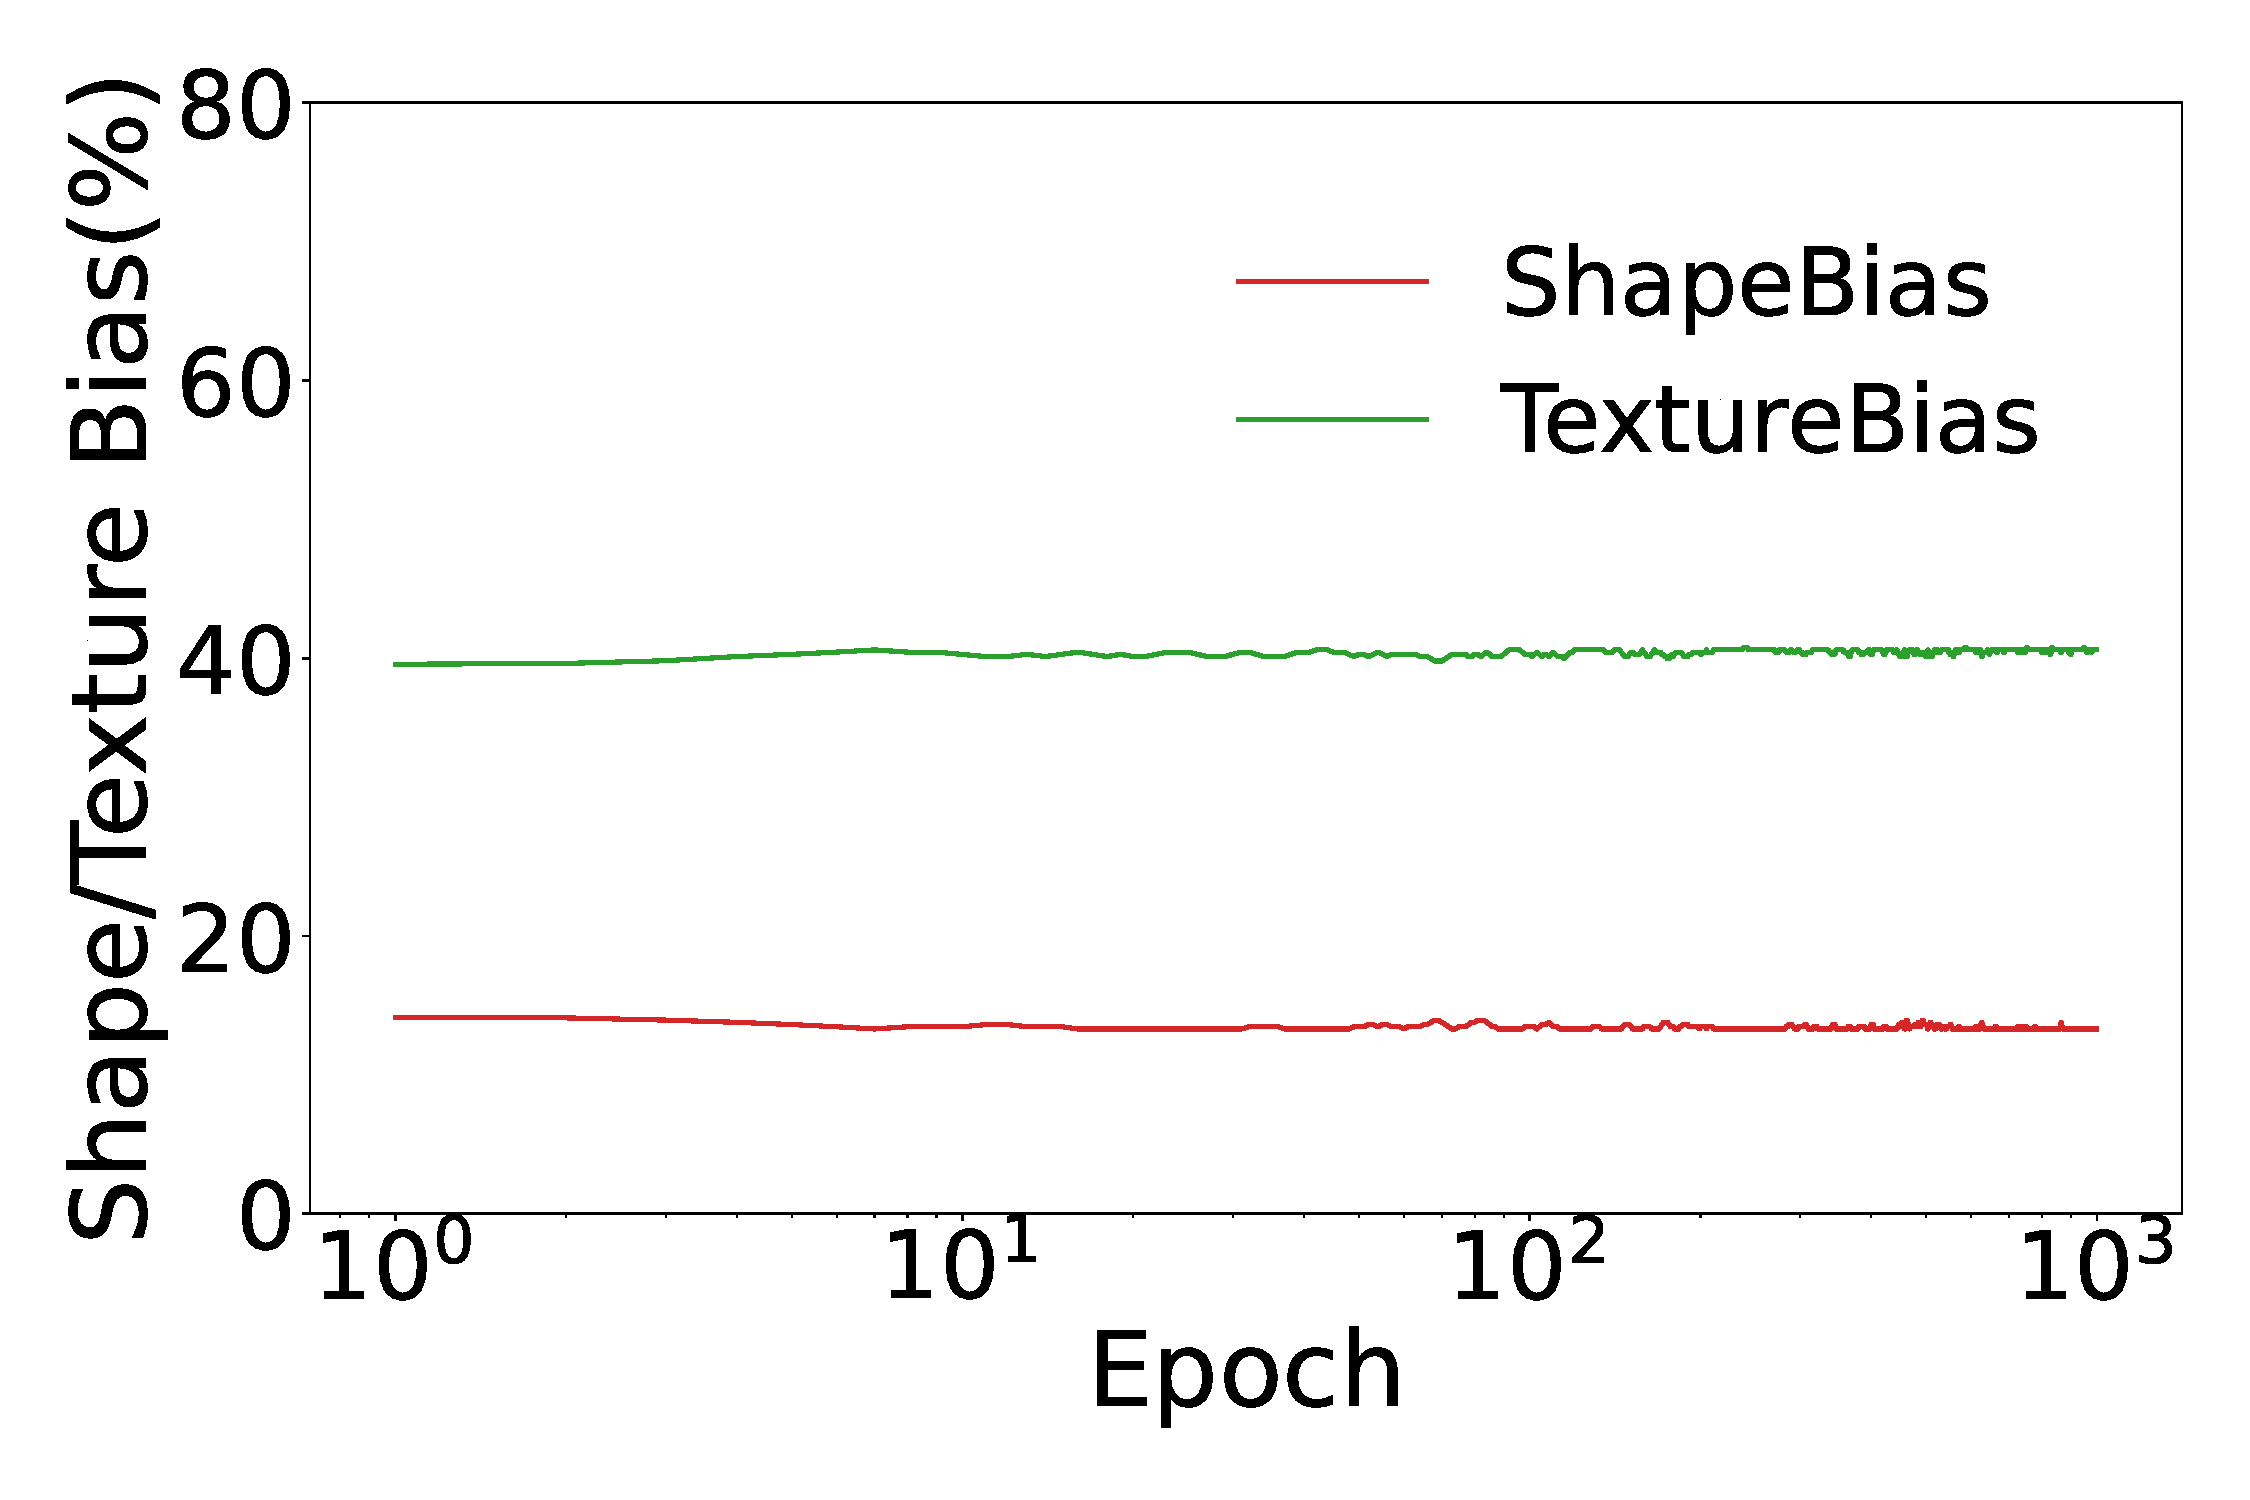
\includegraphics[width=1\linewidth]{bias_fig/IN_ResNet18/layer9.pdf}
    \subcaption{9th layer}% \caption{Figure caption}
  \end{minipage}
\begin{minipage}[b]{.48\linewidth}
    \centering
    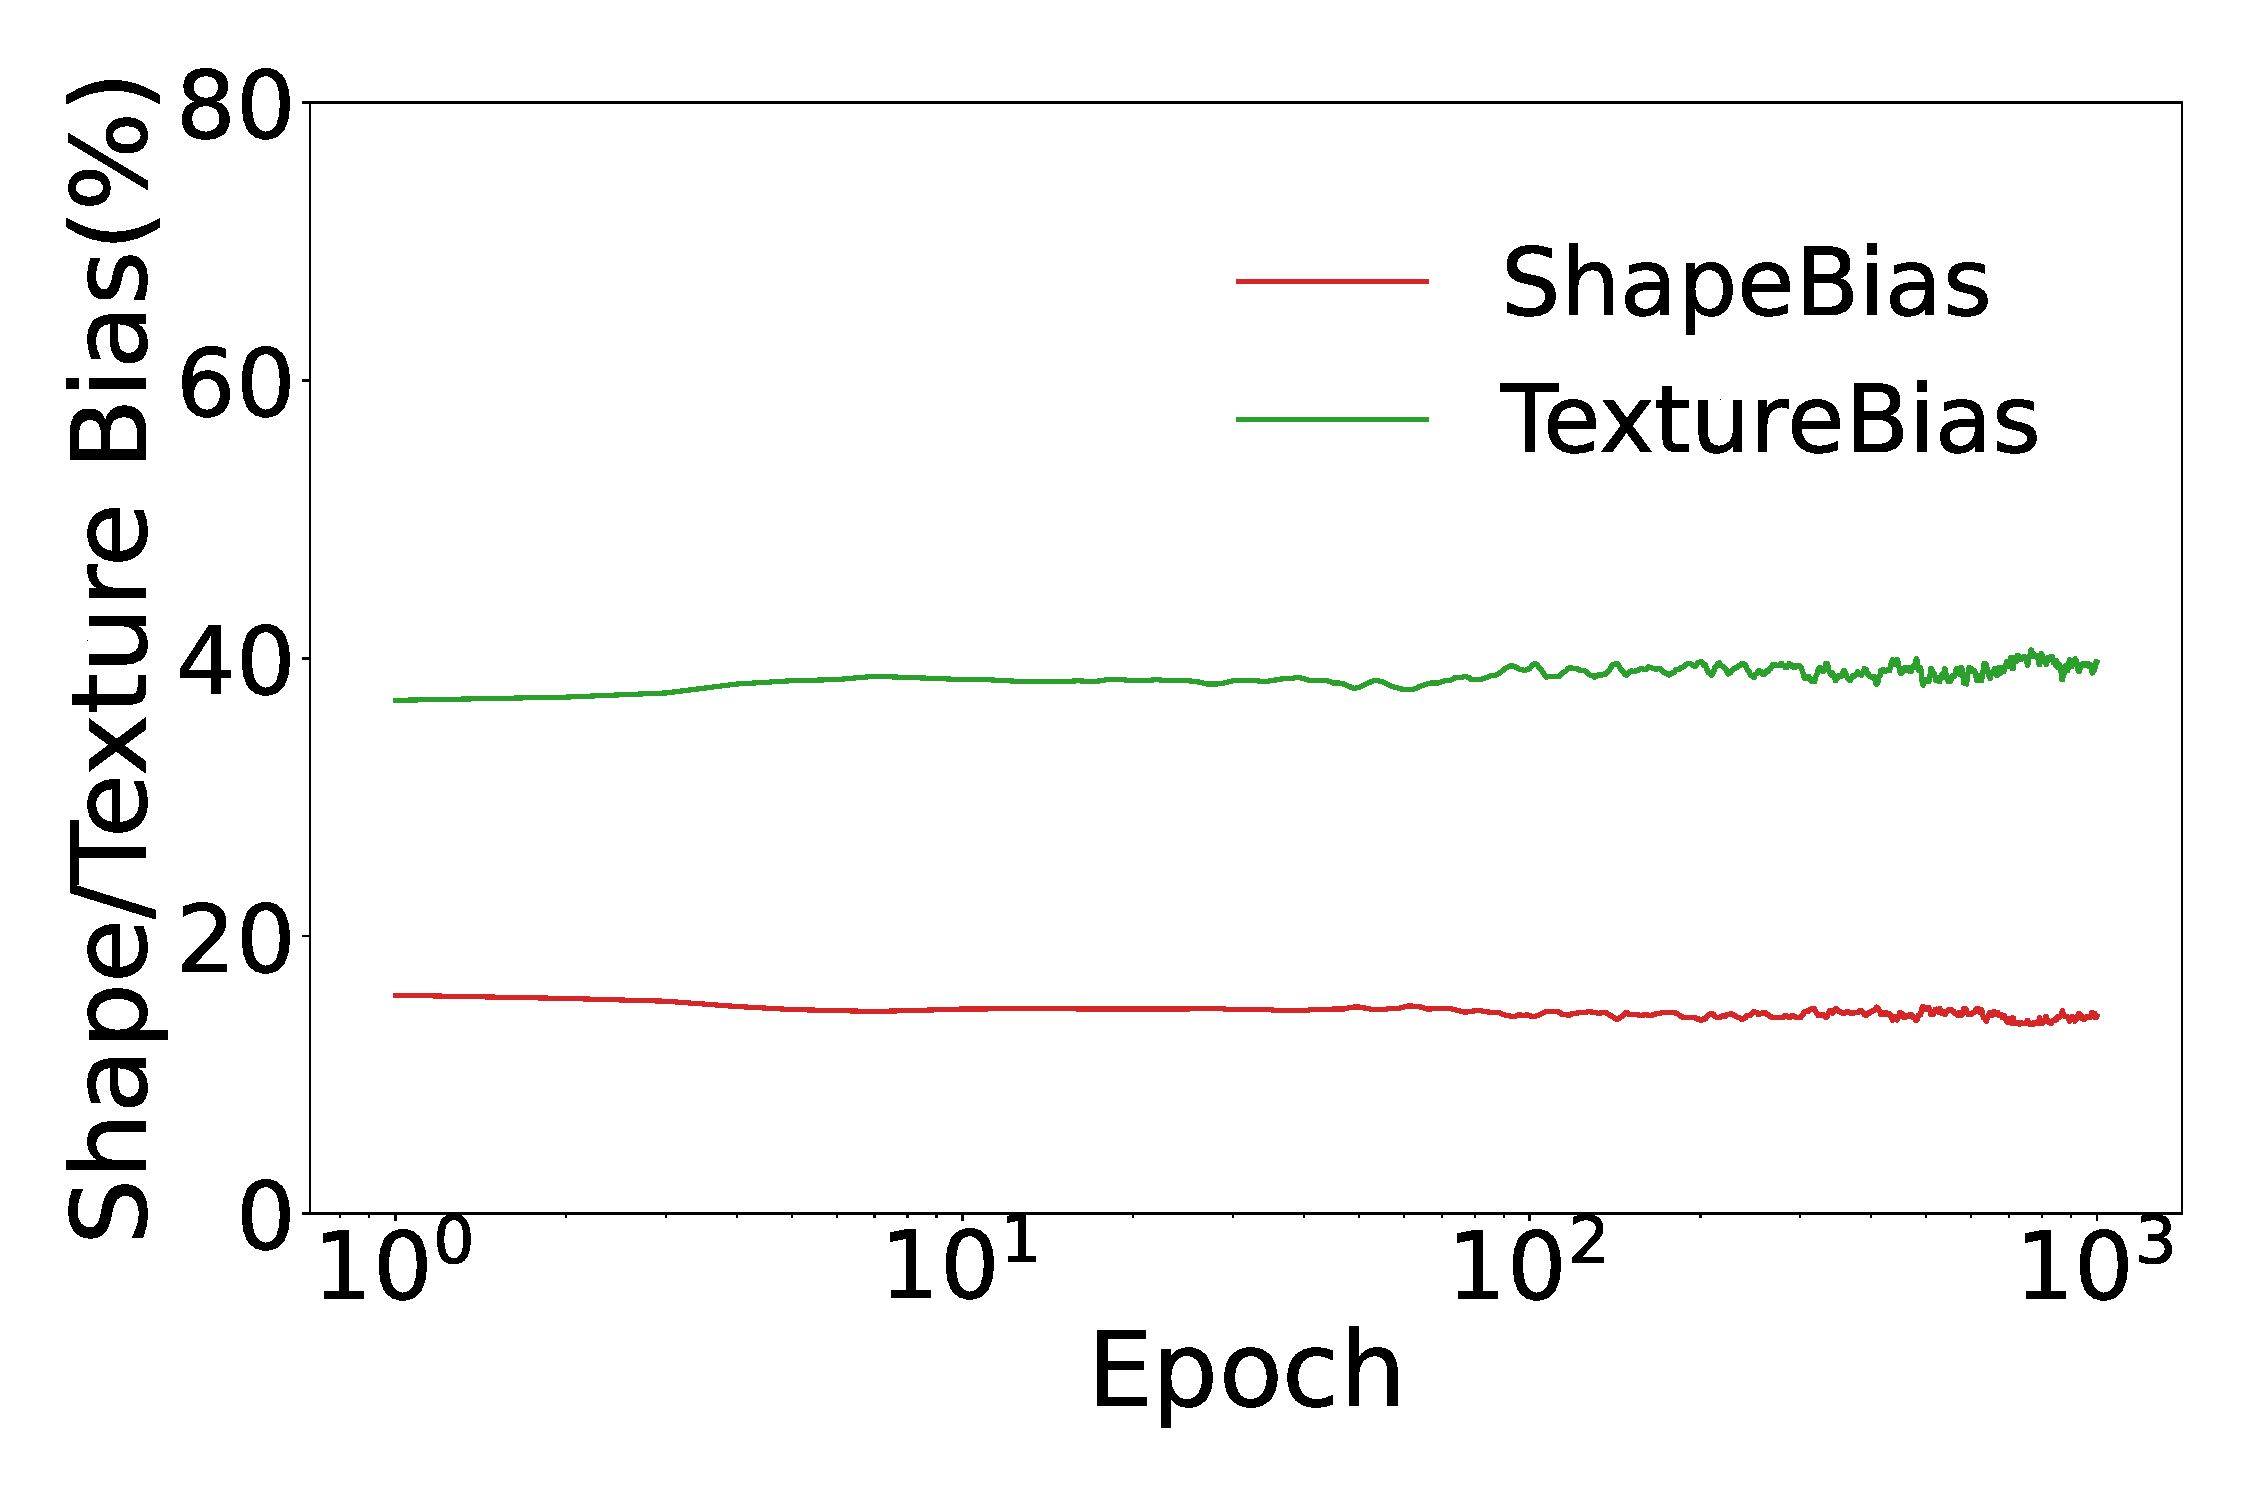
\includegraphics[width=1\linewidth]{bias_fig/IN_ResNet18/layer13.pdf}
    \subcaption{13th layer}% \caption{Figure caption}
  \end{minipage}
\begin{minipage}[b]{.48\linewidth}
    \centering
    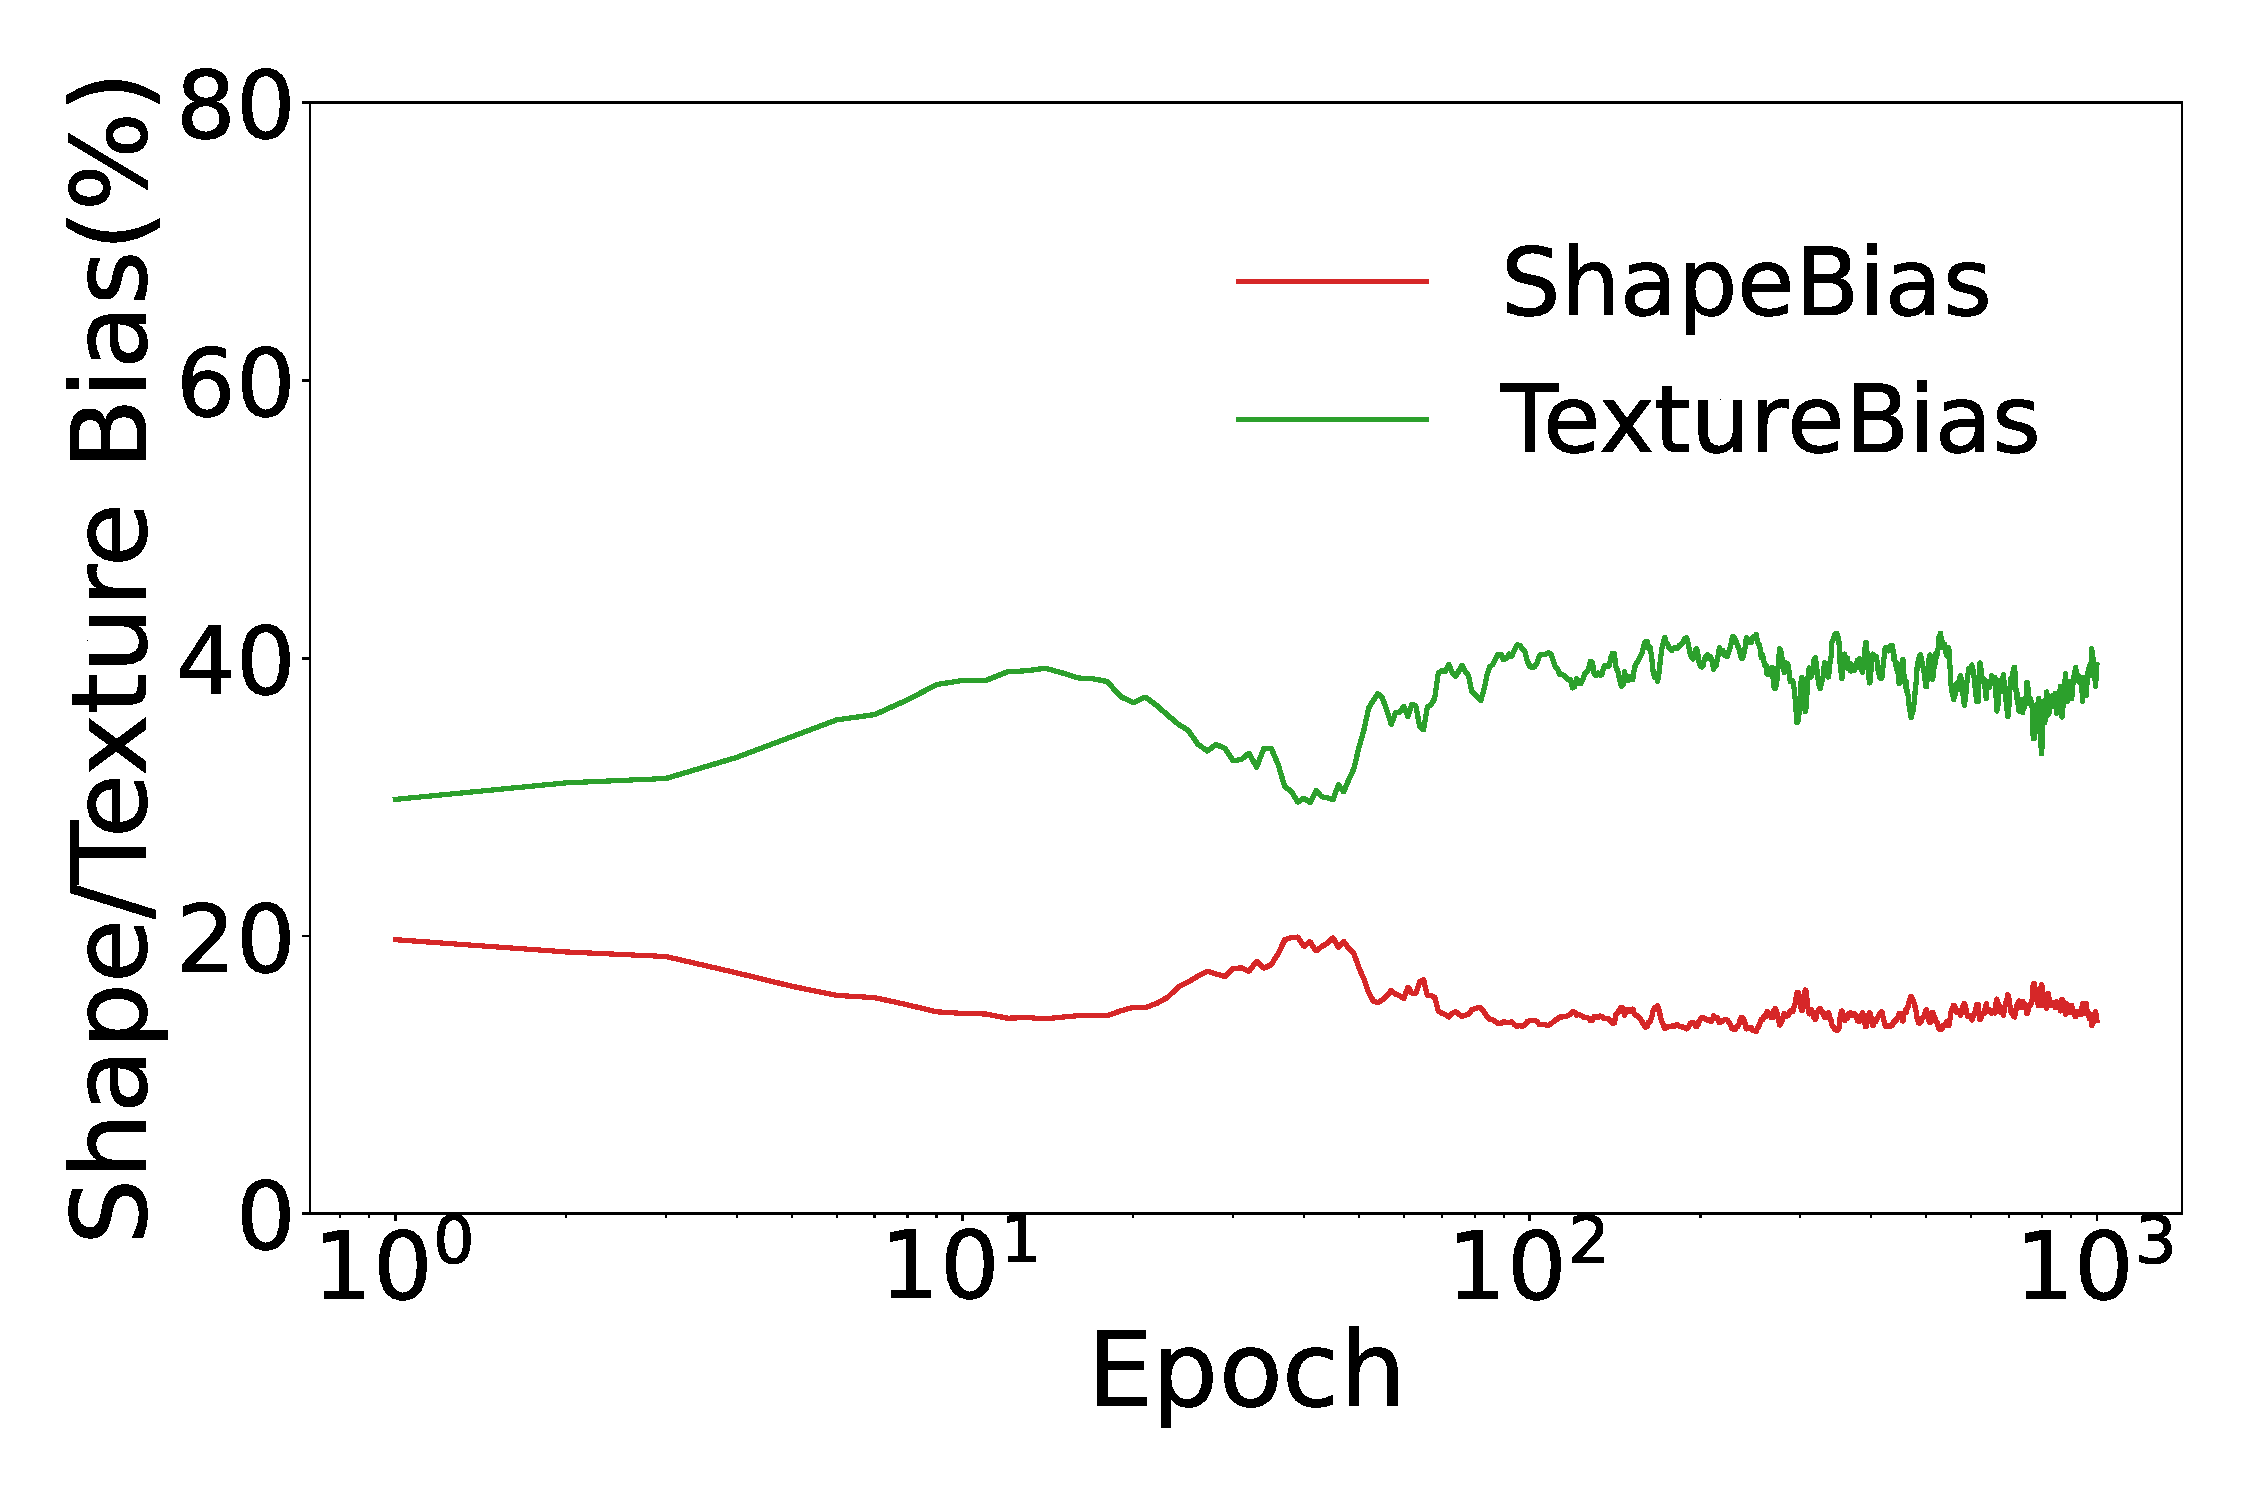
\includegraphics[width=1\linewidth]{bias_fig/IN_ResNet18/layer17.pdf}
    \subcaption{17th layer}% \caption{Figure caption}
  \end{minipage}
\caption{
The shift of biases during the learning process in each layer consisting ResNet18. 
}
\label{fig:layer_ab}
\end{figure}

\newpage

\section{浅い層のカーネル可視化}
前節では,深い層にのみ見られる何らかの特性が存在する可能性が示唆された,一方で,浅い層に変化はないのか,第1層の可視化を通して検証を行った.使用した条件は,前節と同様に,\cref{fig:overview}と同様である.二重降下の推移が切り替わる点であり,Phaseの切り替わりである13,42,そして学習が終わる1,000 epoch目において可視化を行った.

結果を\cref{fig:visualized_kernel}に示す.各フィルターを確認すると,形状テクスチャ偏重度の特異な推移が確認される条件においても,変化は微小である.浅い層の変化は少ないことから,偏重度の特異な推移に,浅い層の学習が関係している可能性は引くと考えられる.また,事前学習したときに収束したパラメータが,浅い層においては,異なるデータセット(今回はCIFAR-10)に対しても有効であったためだと考える.
\begin{figure}[h]
    \centering
    \begin{subfigure}{0.3\textwidth}
        \centering
        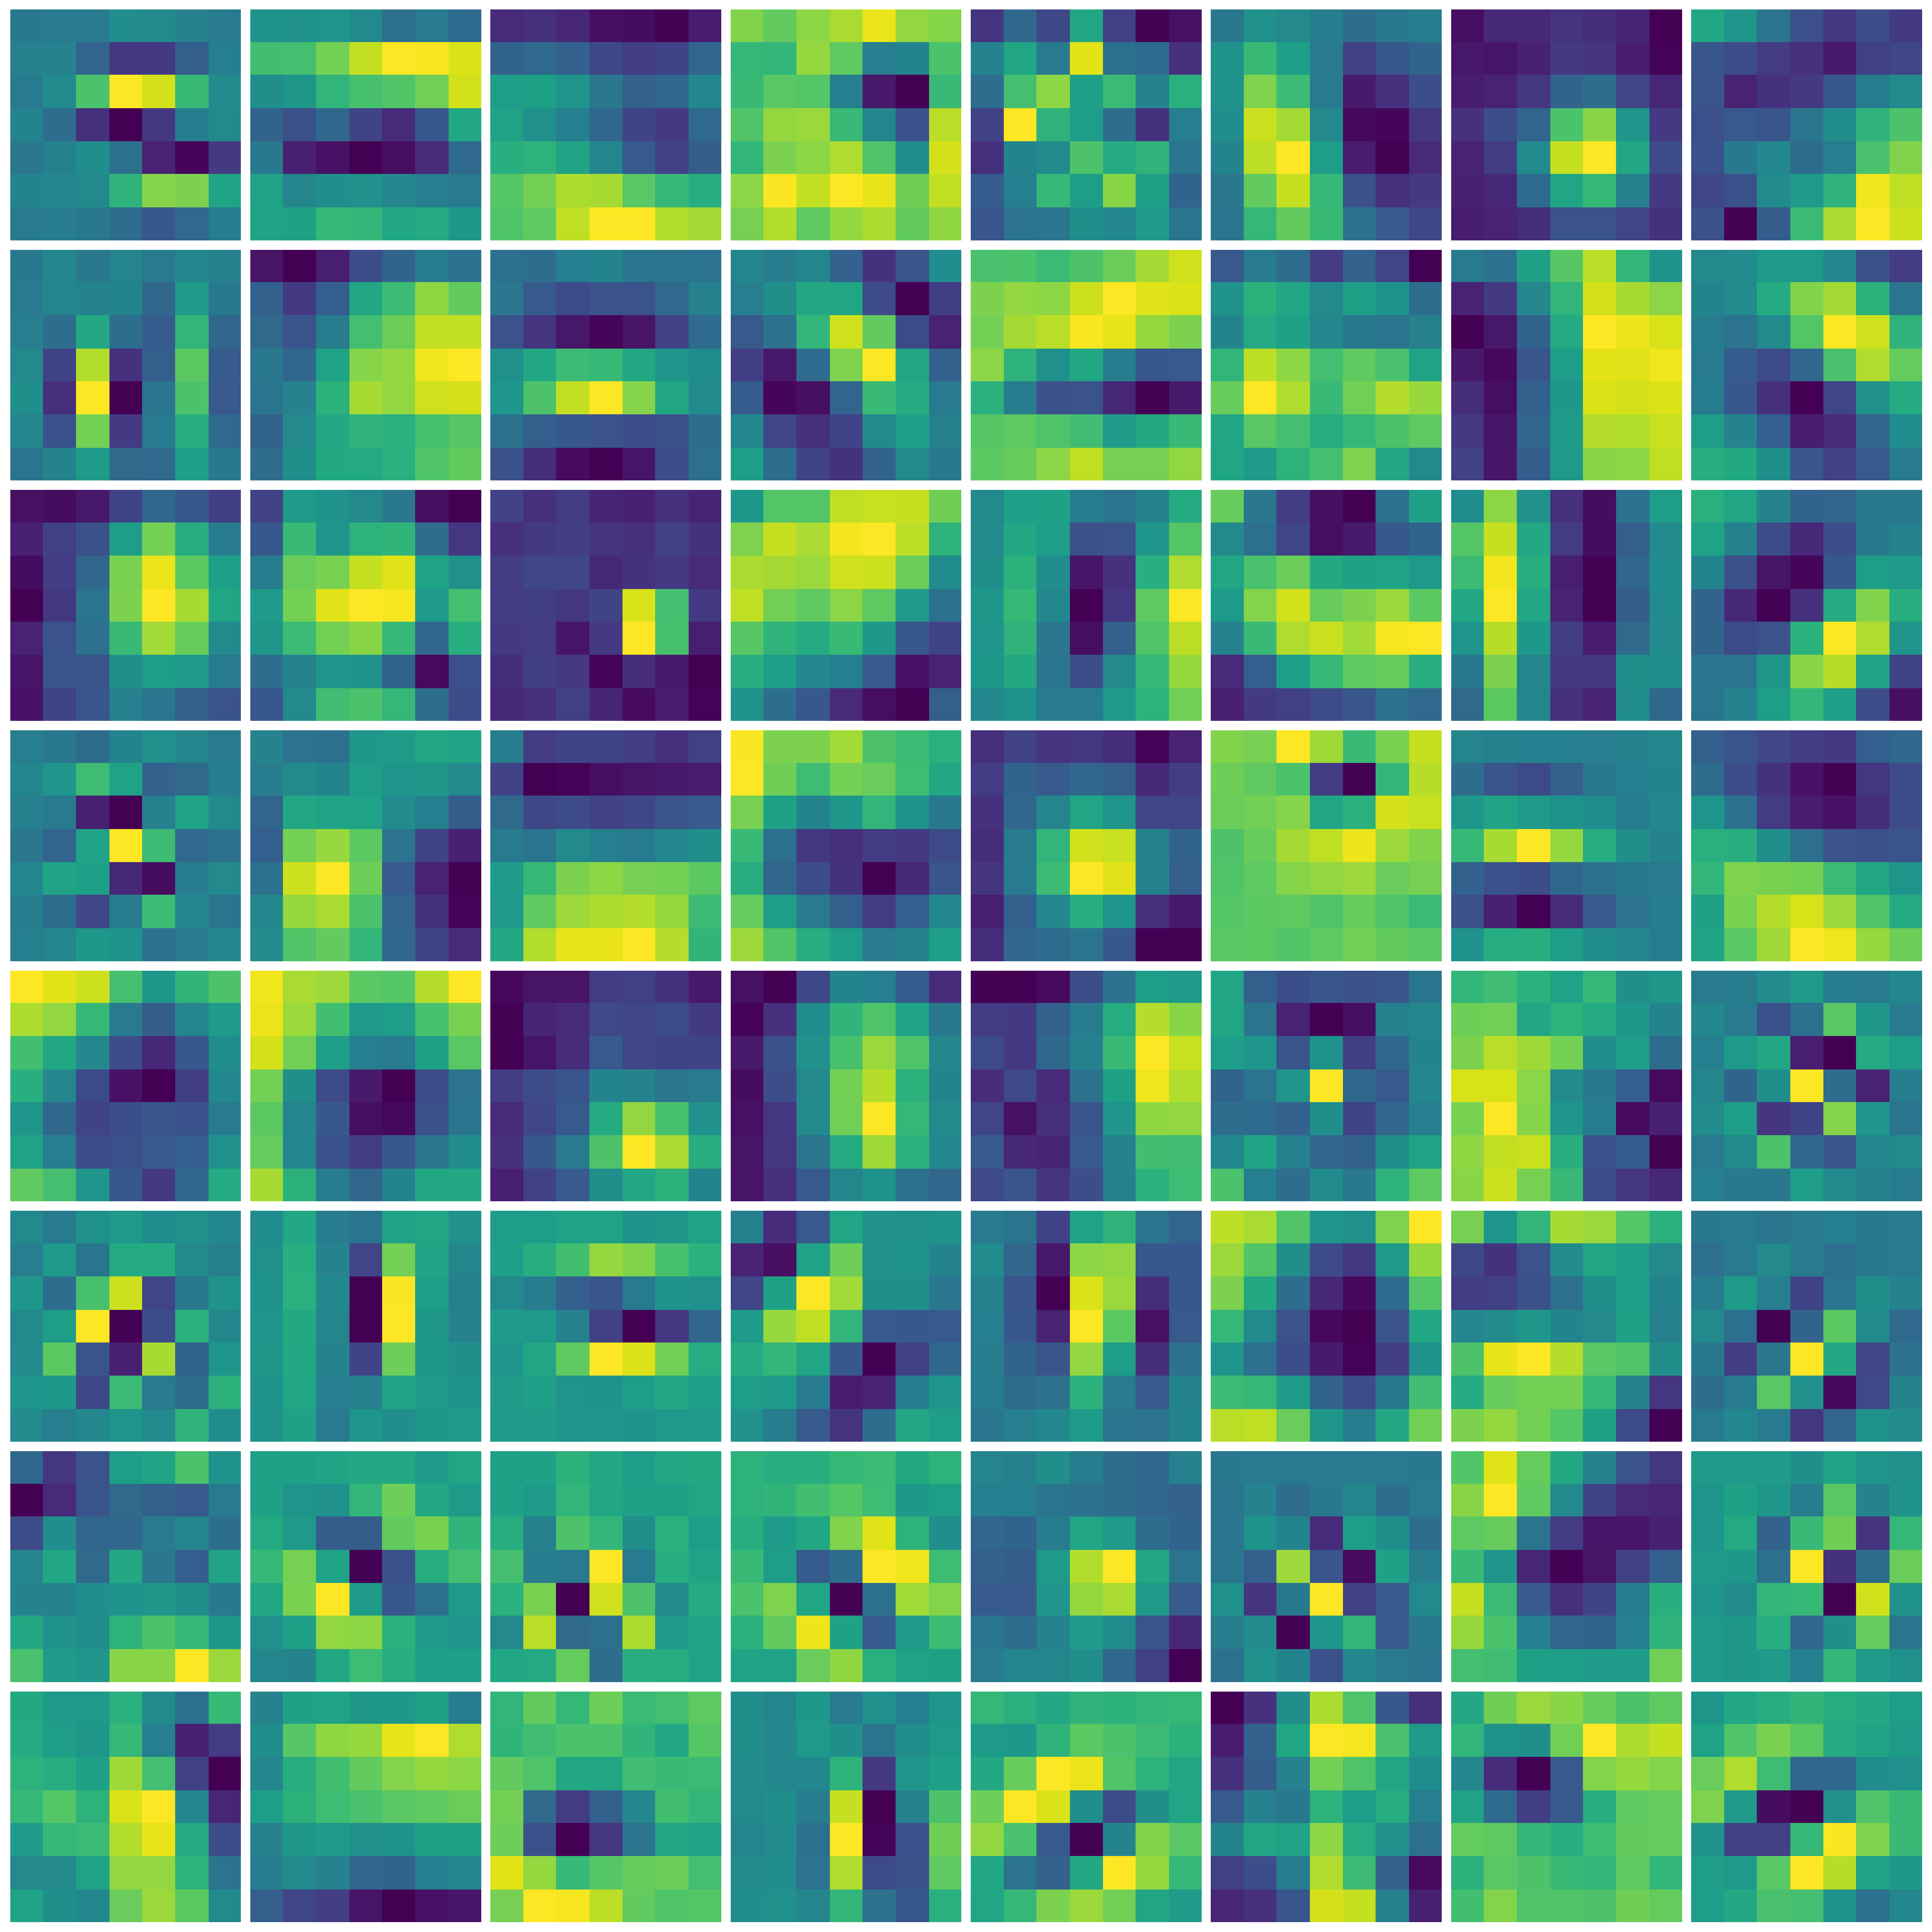
\includegraphics[width=\linewidth]{fig/IN_kernel/Visualize_epoch13.pdf}
        \caption{13th Epoch}
        \label{fig:13th}
    \end{subfigure}
    \begin{subfigure}{0.3\textwidth}
        \centering
        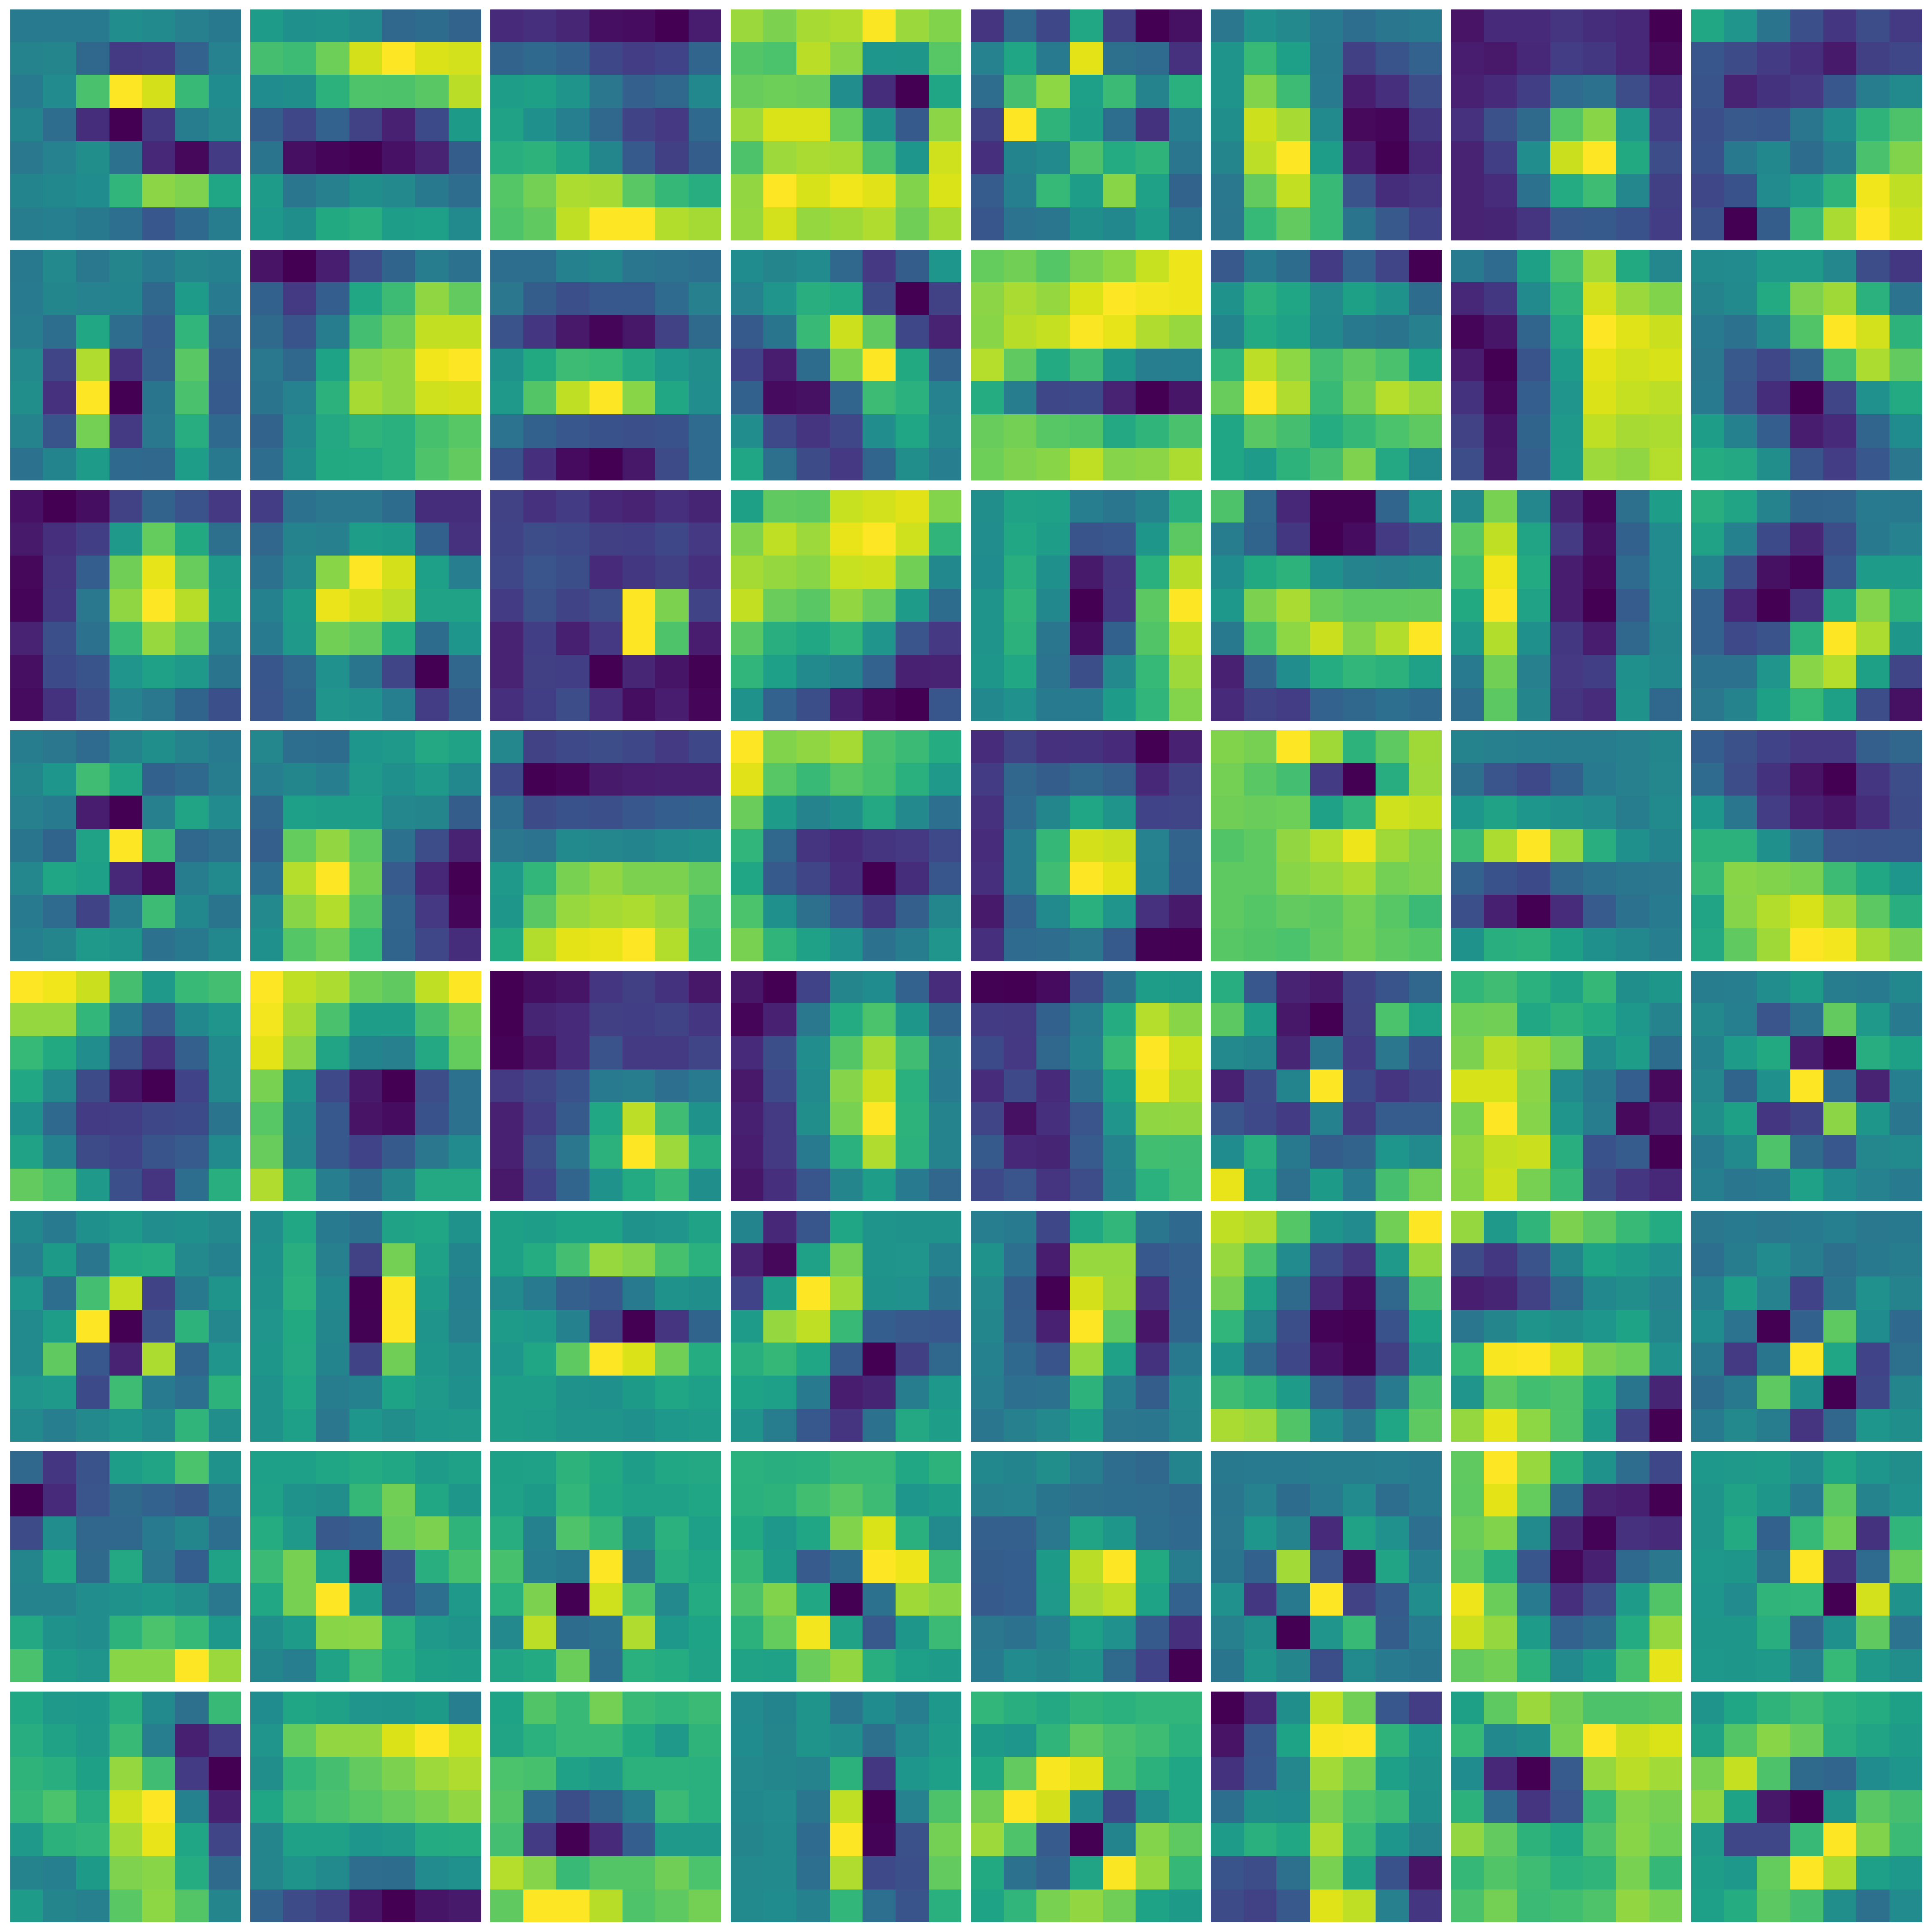
\includegraphics[width=\linewidth]{fig/IN_kernel/Visualize_epoch42.pdf}
        \caption{42nd Epoch}
        \label{fig:42nd}
    \end{subfigure}
    \begin{subfigure}{0.3\textwidth}
        \centering
        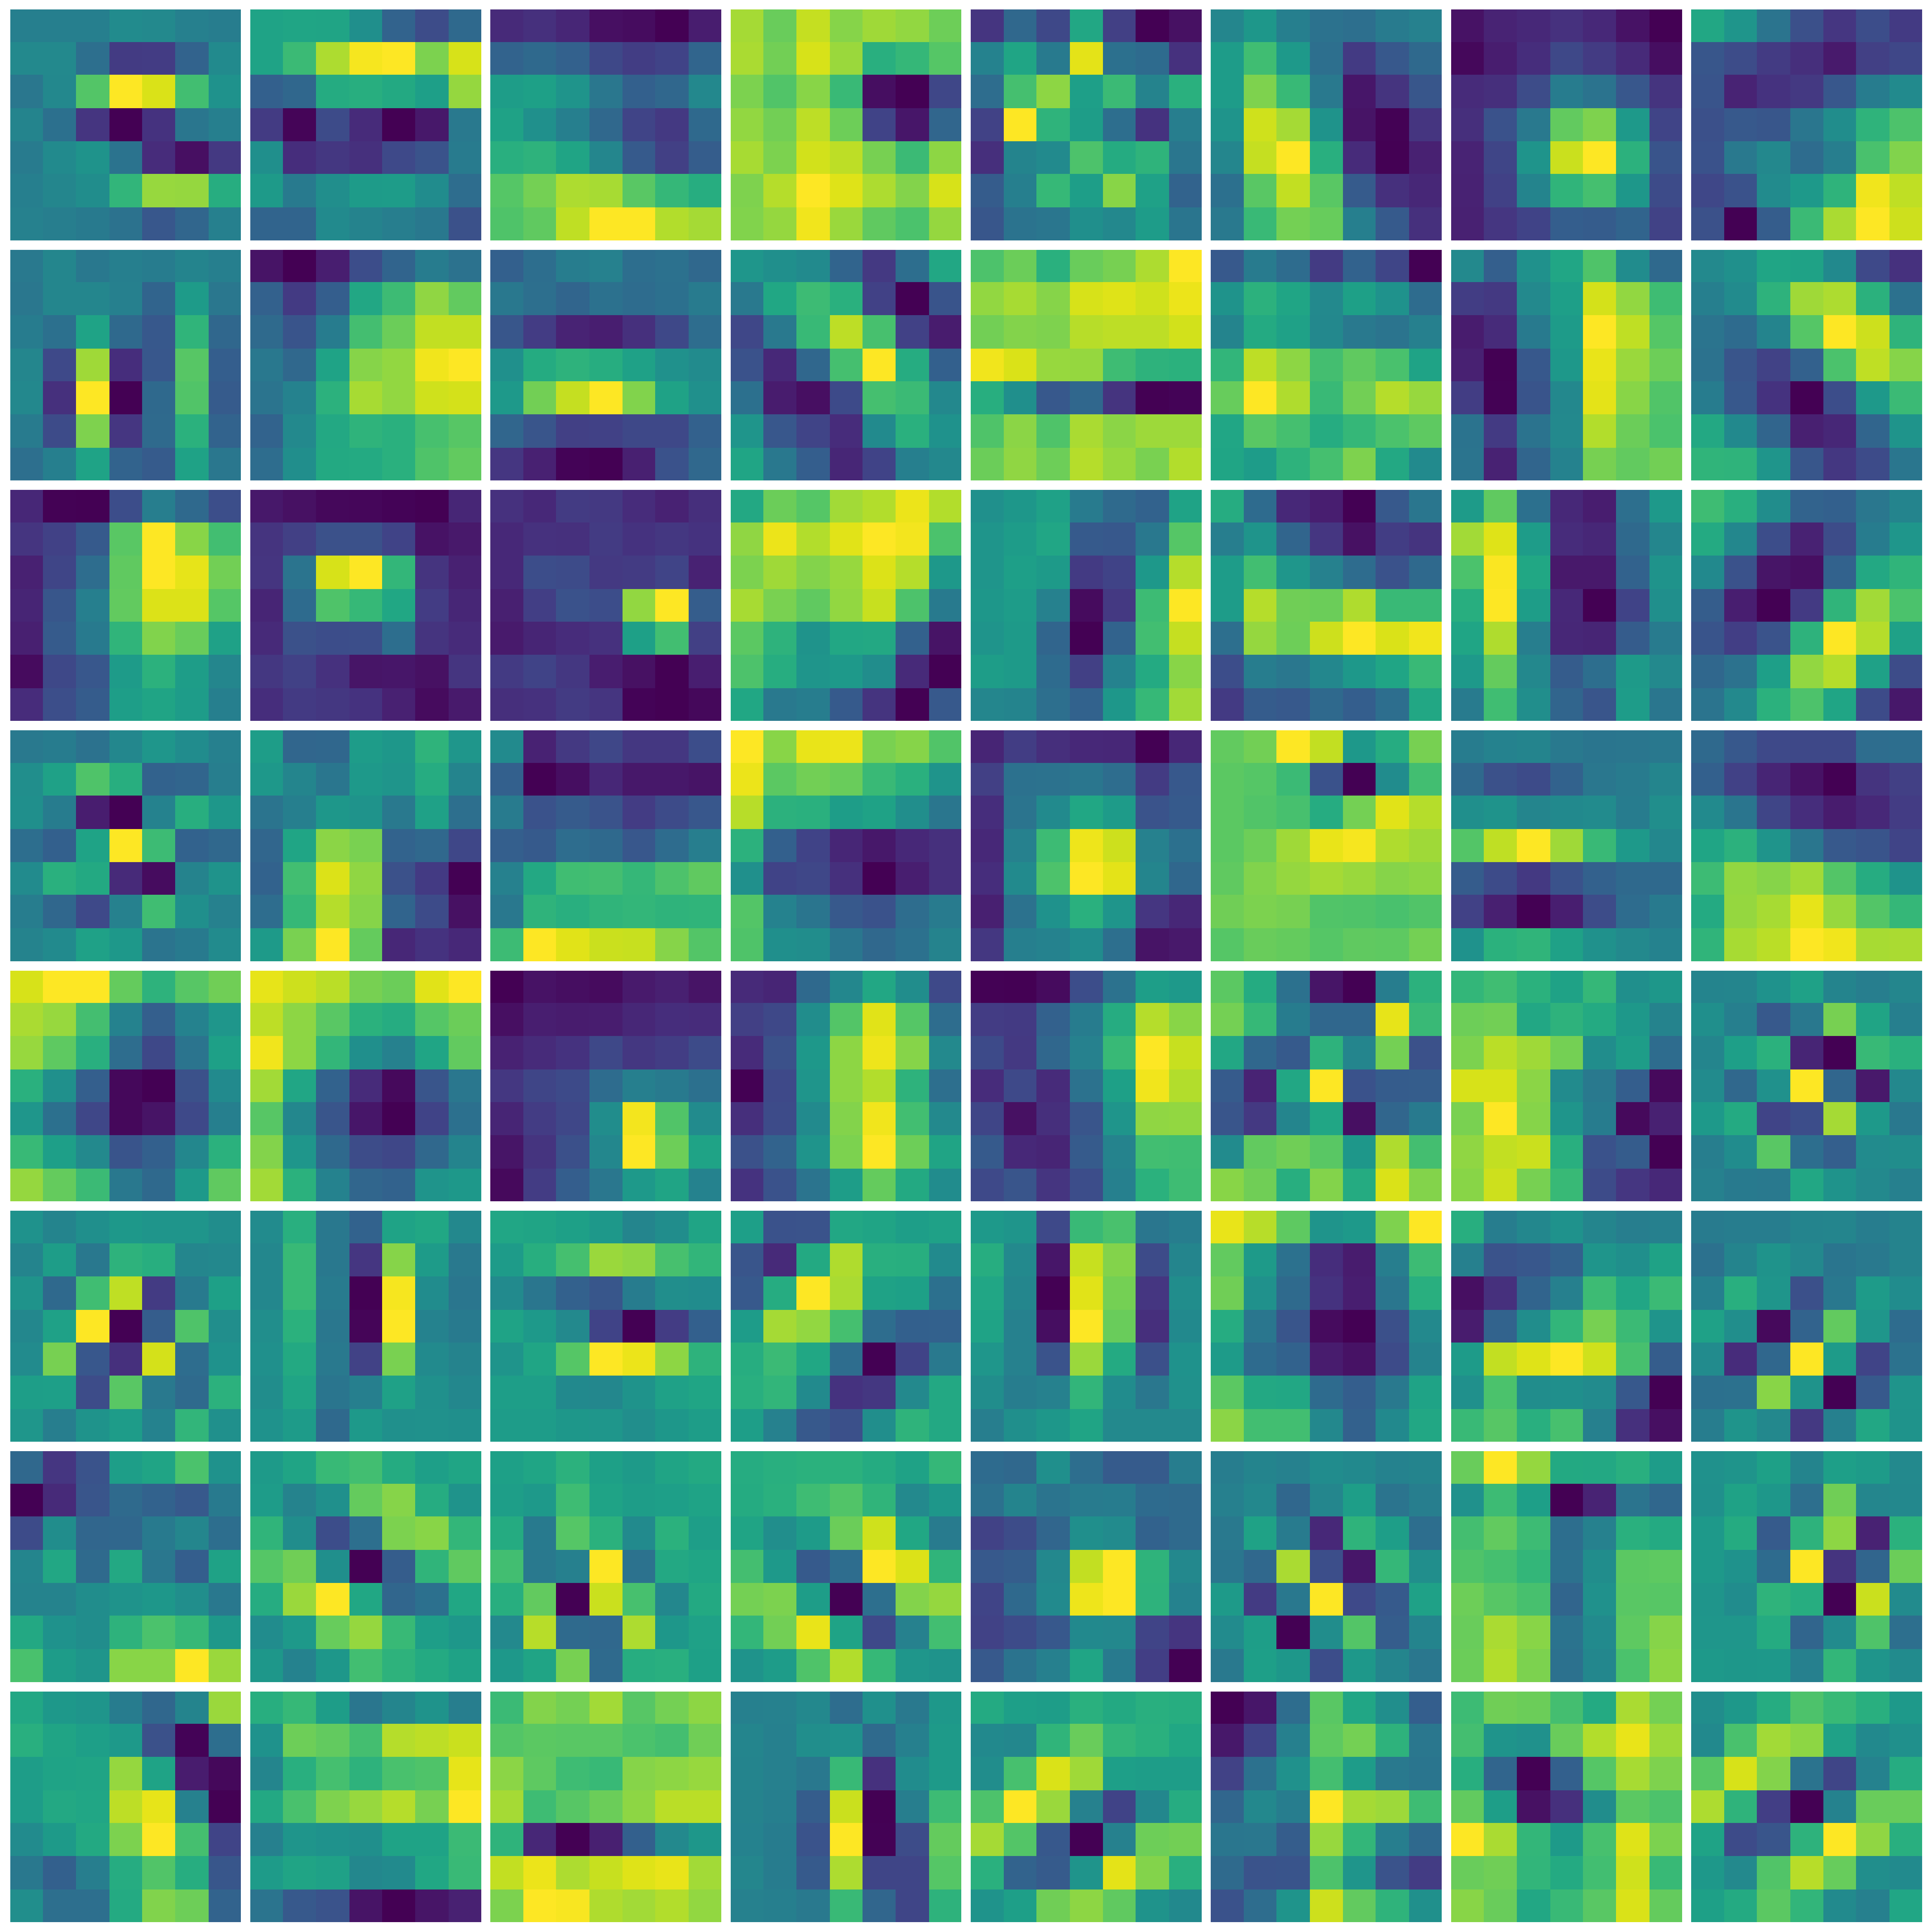
\includegraphics[width=\linewidth]{fig/IN_kernel/Visualize_epoch1000.pdf}
        \caption{1,000th Epoch}
        \label{fig:1000th}
    \end{subfigure}
    \caption[Visualization of the 1st layer in the learning process.]{
    % 学習過程における1st layerの可視化.\cref{sec:Experimental setting}で説明した設定において,二重降下を3つのPhaseに分割するEpoch(13th, 42nd Epoch),1,000th Epochにおける1st layerを可視化している.
    Visualization of the 1st layer in the learning process. In the setting described in Sec. 5.2, we visualize the 1st layer in the Epoch (13th, 42nd Epoch) and the 1,000th Epoch, where the double descent is divided into 3 Phases. The 1st layer at the 1,000th Epoch is visualized.
    }
    \label{fig:visualized_kernel}
\end{figure}

\newpage

\section{ブロック凍結実験}
深い層,浅い層における学習時の性質がそれぞれ二重降下と形状テクスチャ偏重度にどのように影響するかを観察するため,モデルが持つパラメータを凍結して,\cref{fig:overview}と同様に実験を行った.パラメータの凍結は,指定した層のパラメータを更新しないというものである.
深い層から順に凍結した場合の結果を\cref{fig:comp_frozen_deep_layer}に示す.深い層から凍結するパラメータを増加させていくと,二重降下の曲線は著しく変化が見られる.それに対して,形状テクスチャ偏重度は,特にfcからblock3を凍結した場合に,二重降下の下降から上昇に移り変わる部分と同期しているように見られる.
浅い層から順に凍結した場合の結果を\cref{fig:comp_frozen_shallow_layer}に示す.この場合は二重降下の曲線はほぼ一致しており,形状・テクスチャ偏重度の推移も類似点が確認できる.
このような結果から,深い層のパラメータが学習される場合,浅い層よりも,二重降下などに対して強い影響を与えていると考えられる.

\begin{figure}[htb]
\centering
   \begin{tabular}{cc}
      %---- 最初の図 ---------------------------
      \hspace{-5mm}
      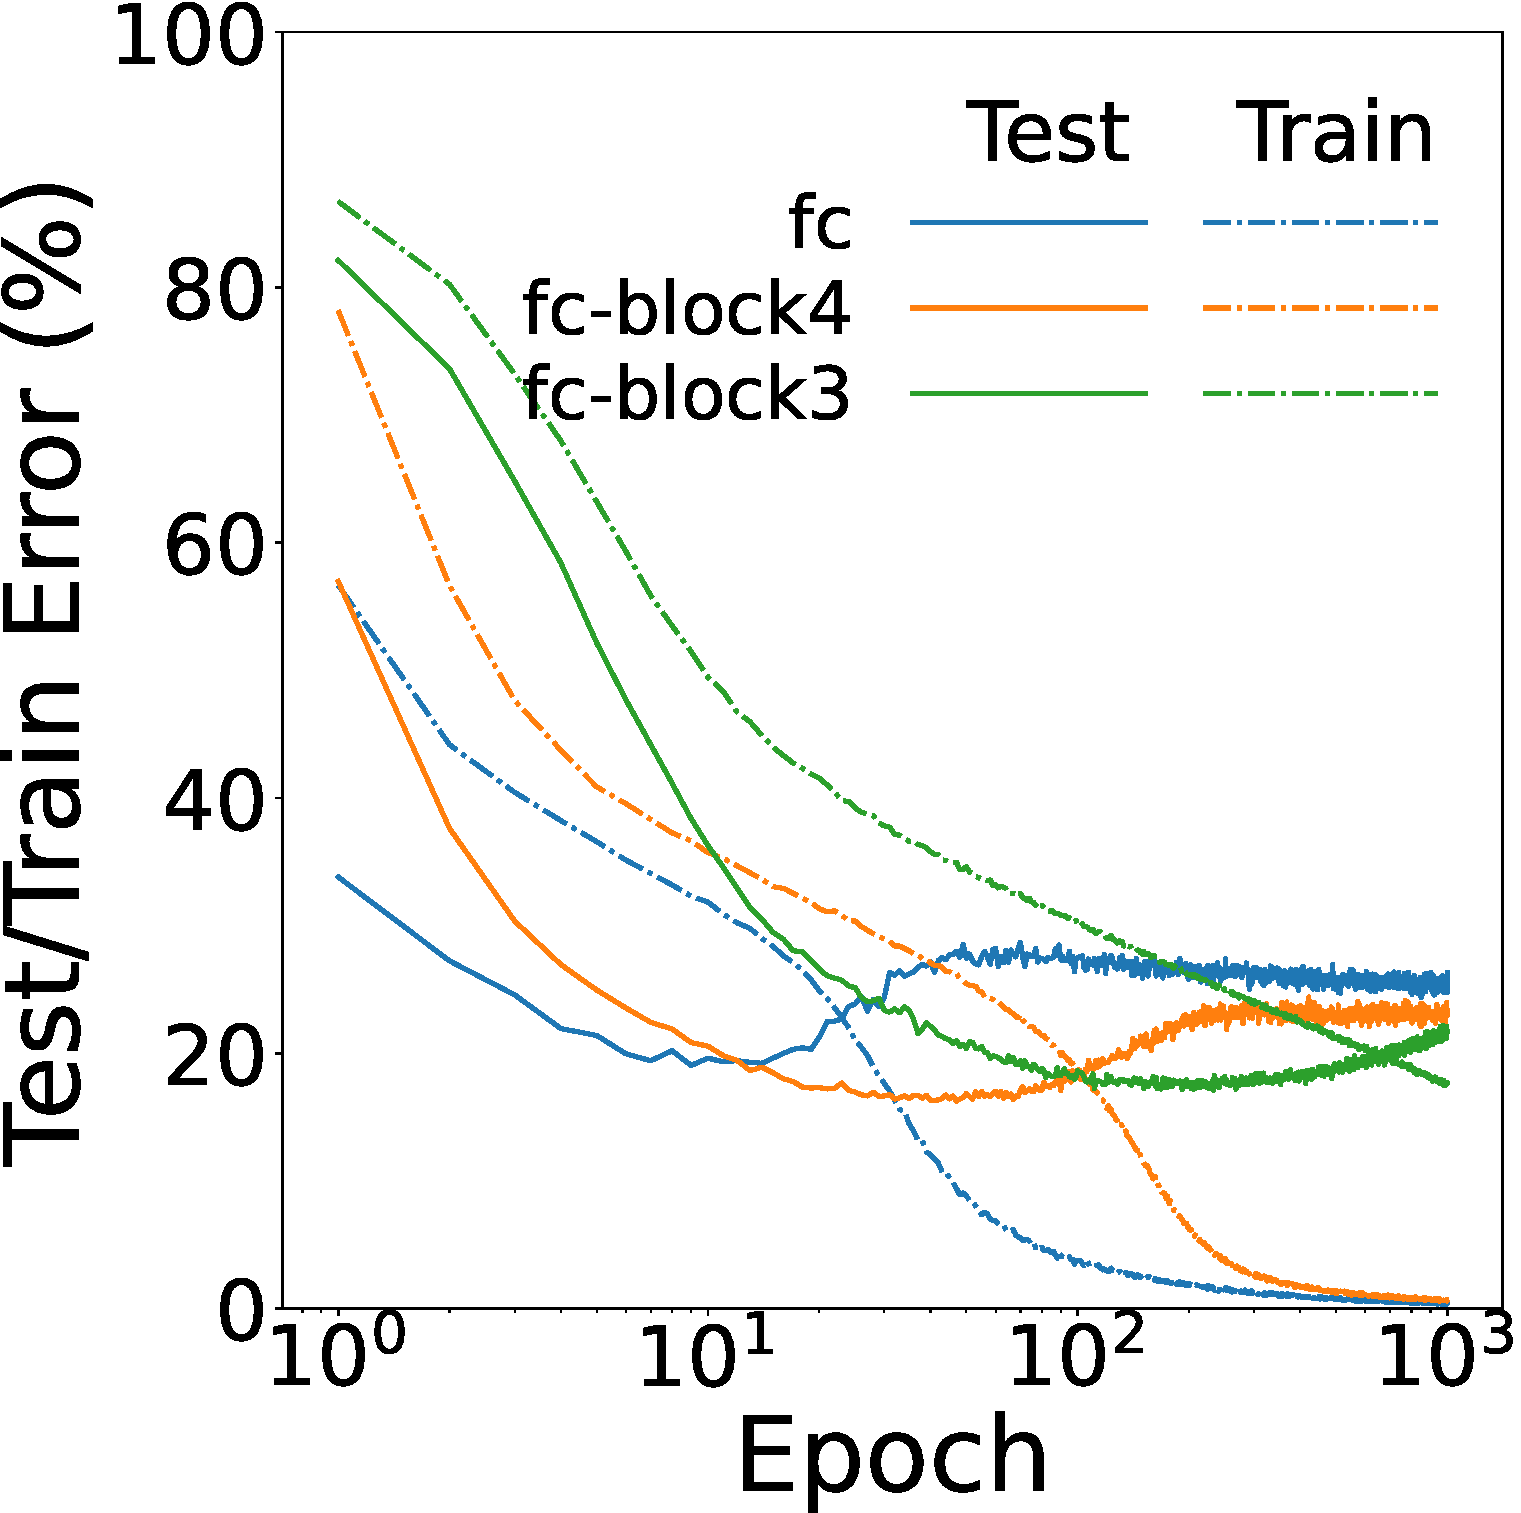
\includegraphics[keepaspectratio, width=0.45\linewidth]{fig/frozen_deep_layer_learning_curv.pdf} &
        \hspace{5pt} 
      %---- 2番目の図 --------------------------
      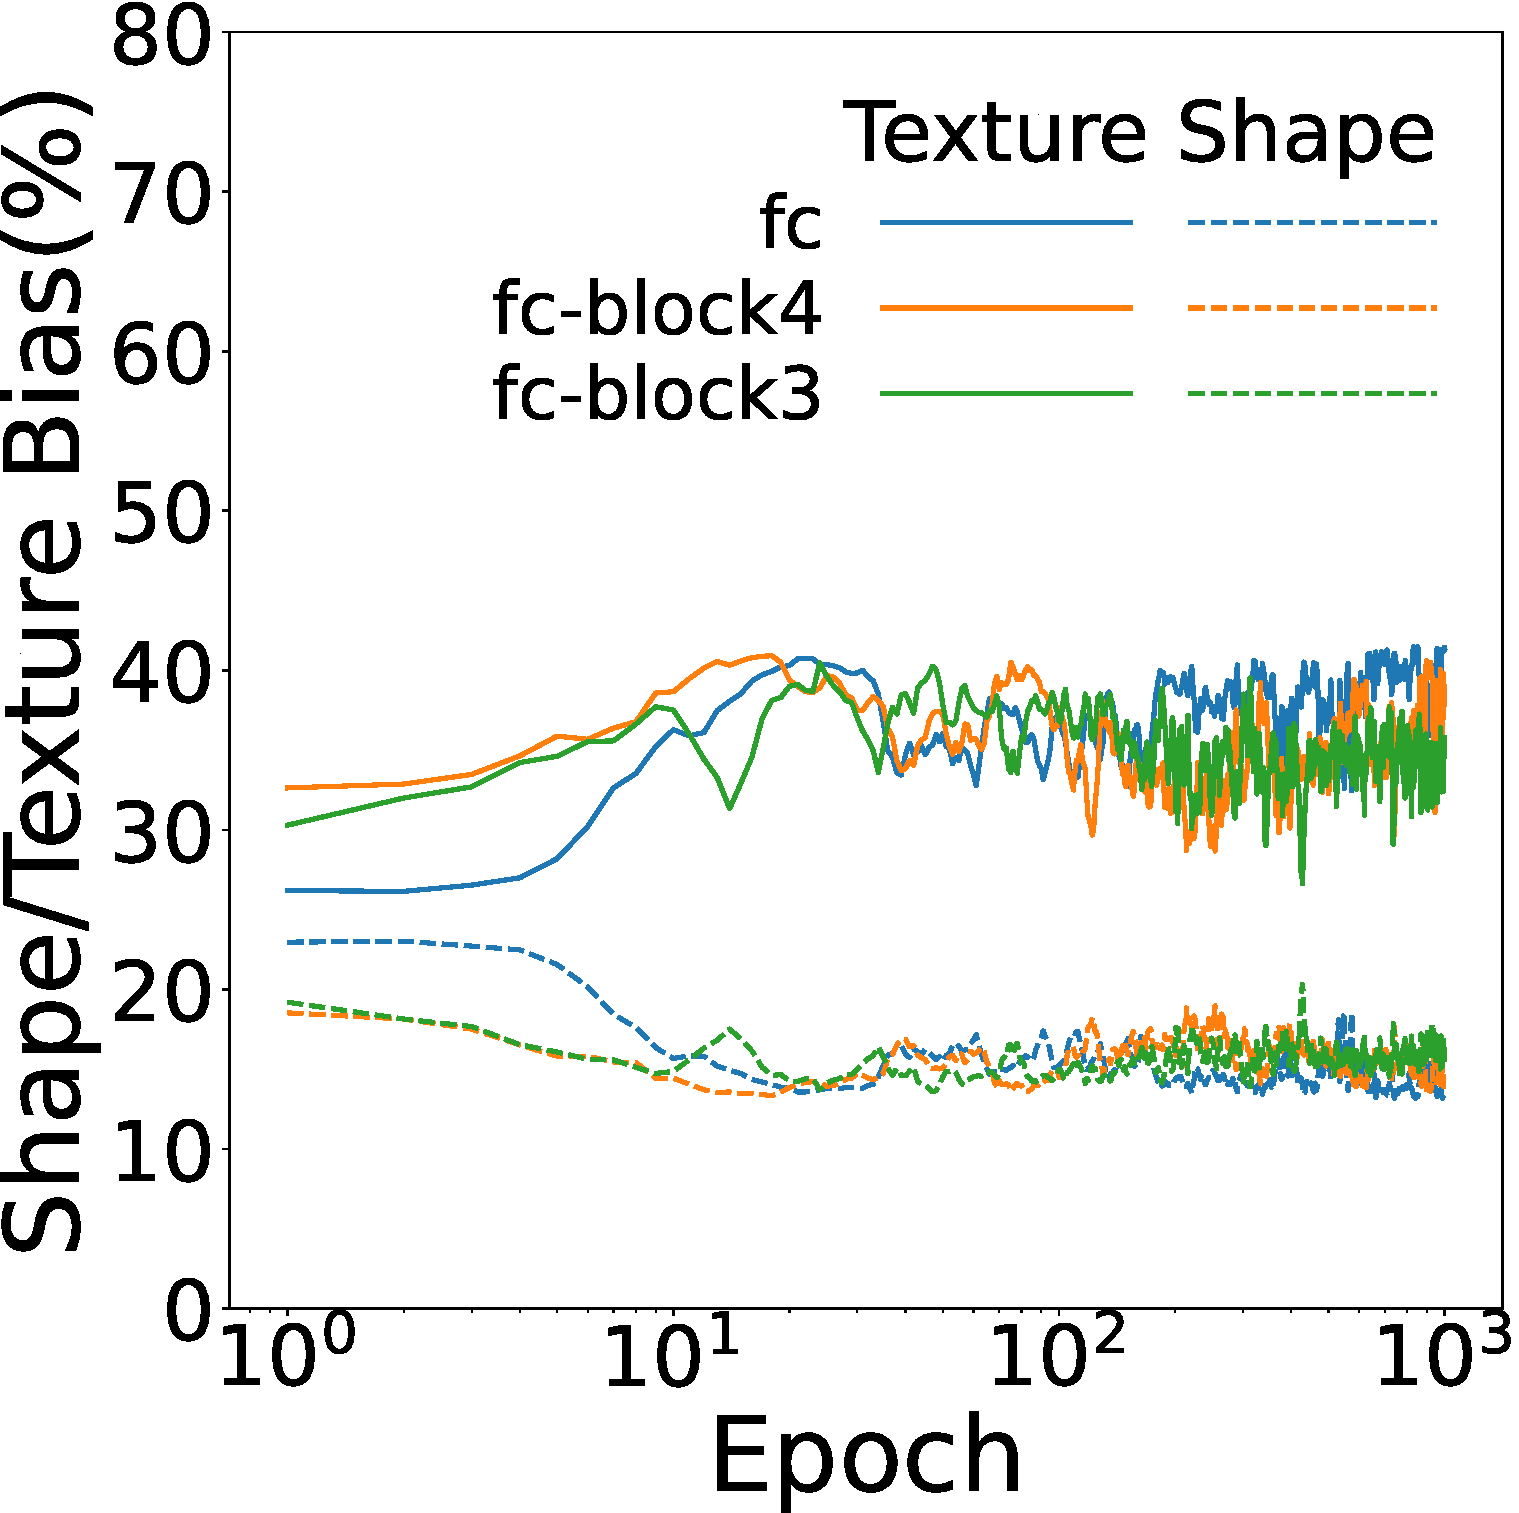
\includegraphics[keepaspectratio, width=0.45\linewidth]{fig/frozen_deep_layer_sha_tex.pdf}
   \end{tabular}
\caption[Learning processes under deep layer parameter freezes.]{Learning processes under deep layer parameter freezes. Left: train/test errors Right: shape/texture bias values.}
%Learning curve graphs for double descent and shape/texture bias for different label noise. \textbf{Left}:learning curve. \textbf{Right}:model's bias shift.}
\label{fig:comp_frozen_deep_layer}
\end{figure}

\begin{figure}[htb]
\centering
   \begin{tabular}{cc}
      %---- 最初の図 ---------------------------
      \hspace{-5mm}
      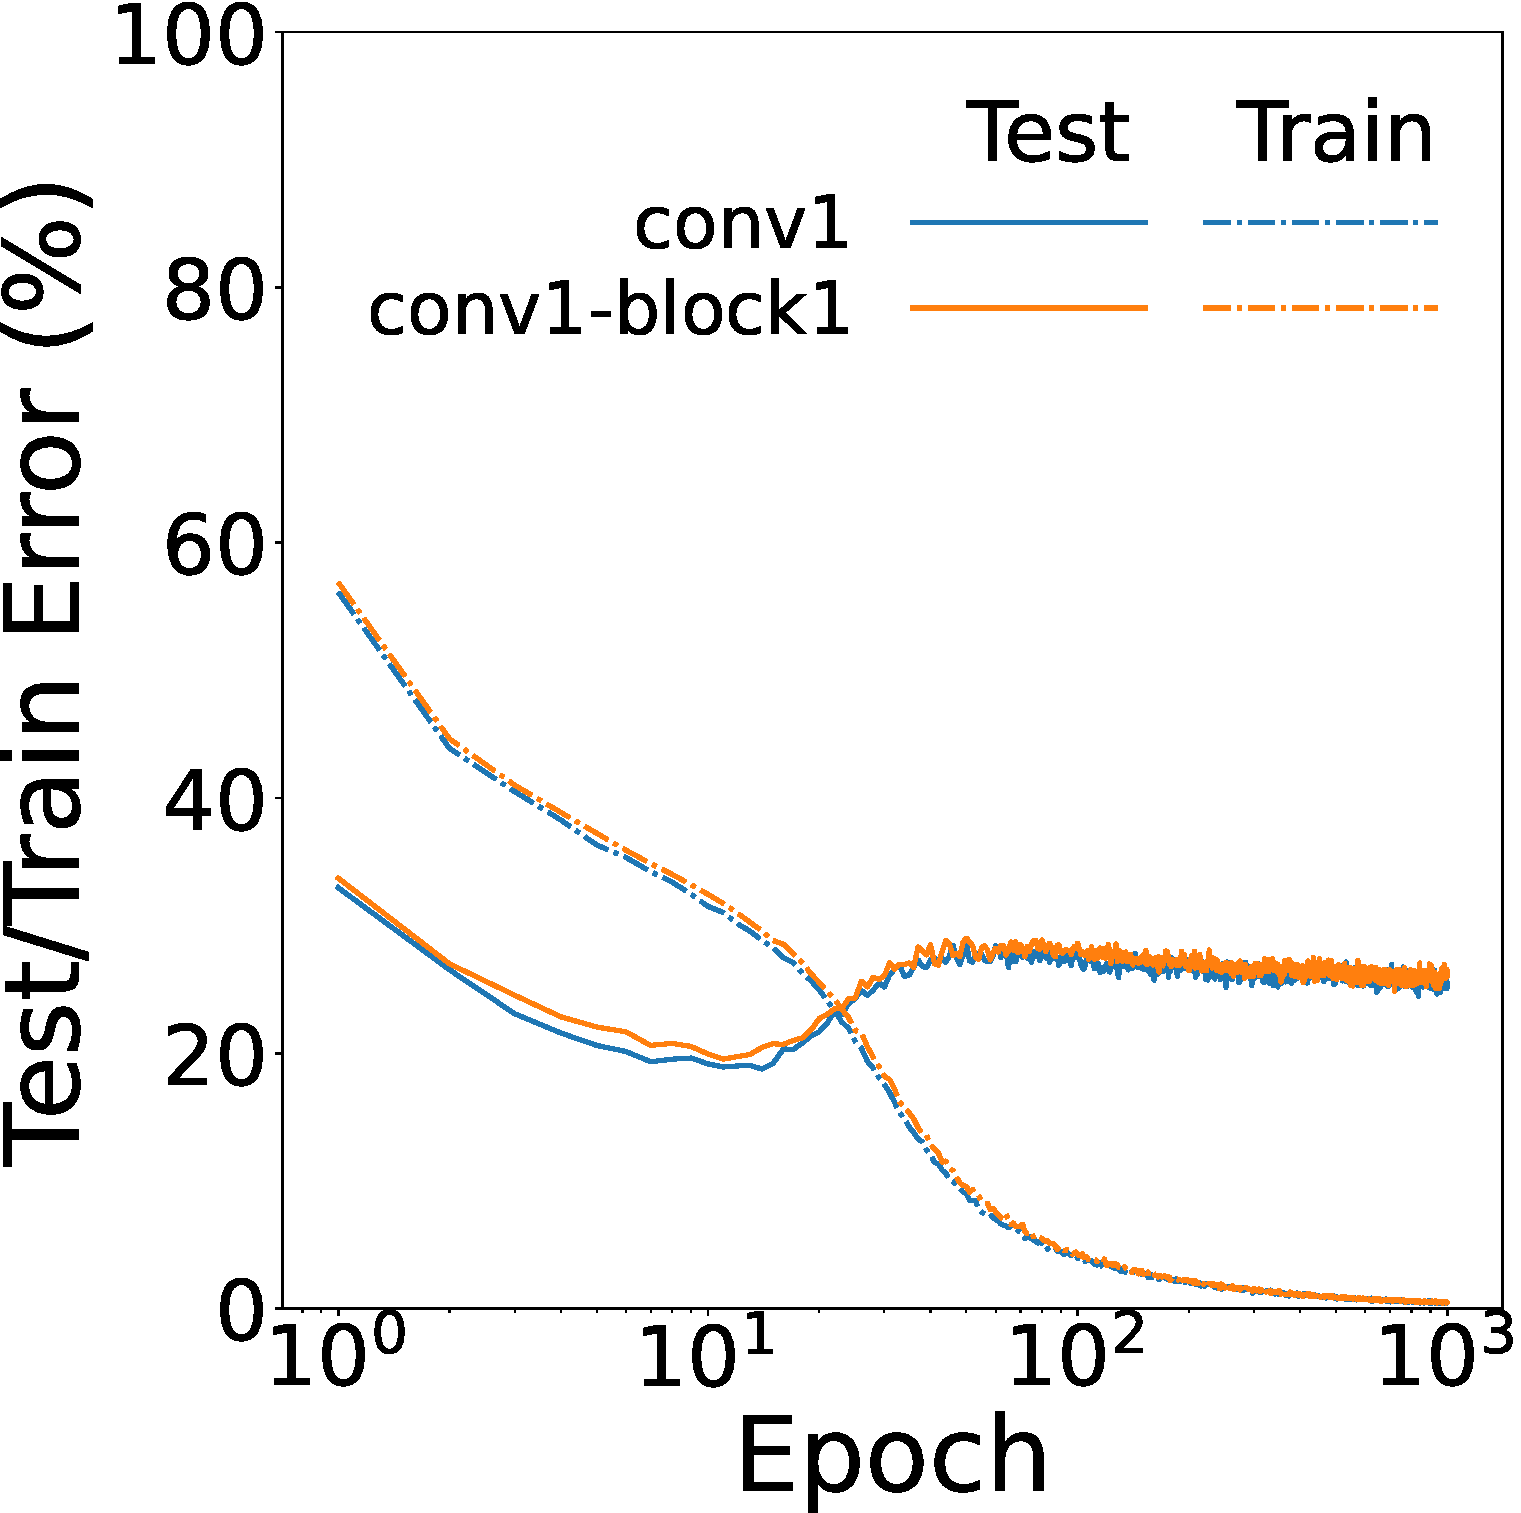
\includegraphics[keepaspectratio, width=0.45\linewidth]{fig/frozen_shallow_layer_learning_curv.pdf} &
        \hspace{5pt} 
      %---- 2番目の図 --------------------------
      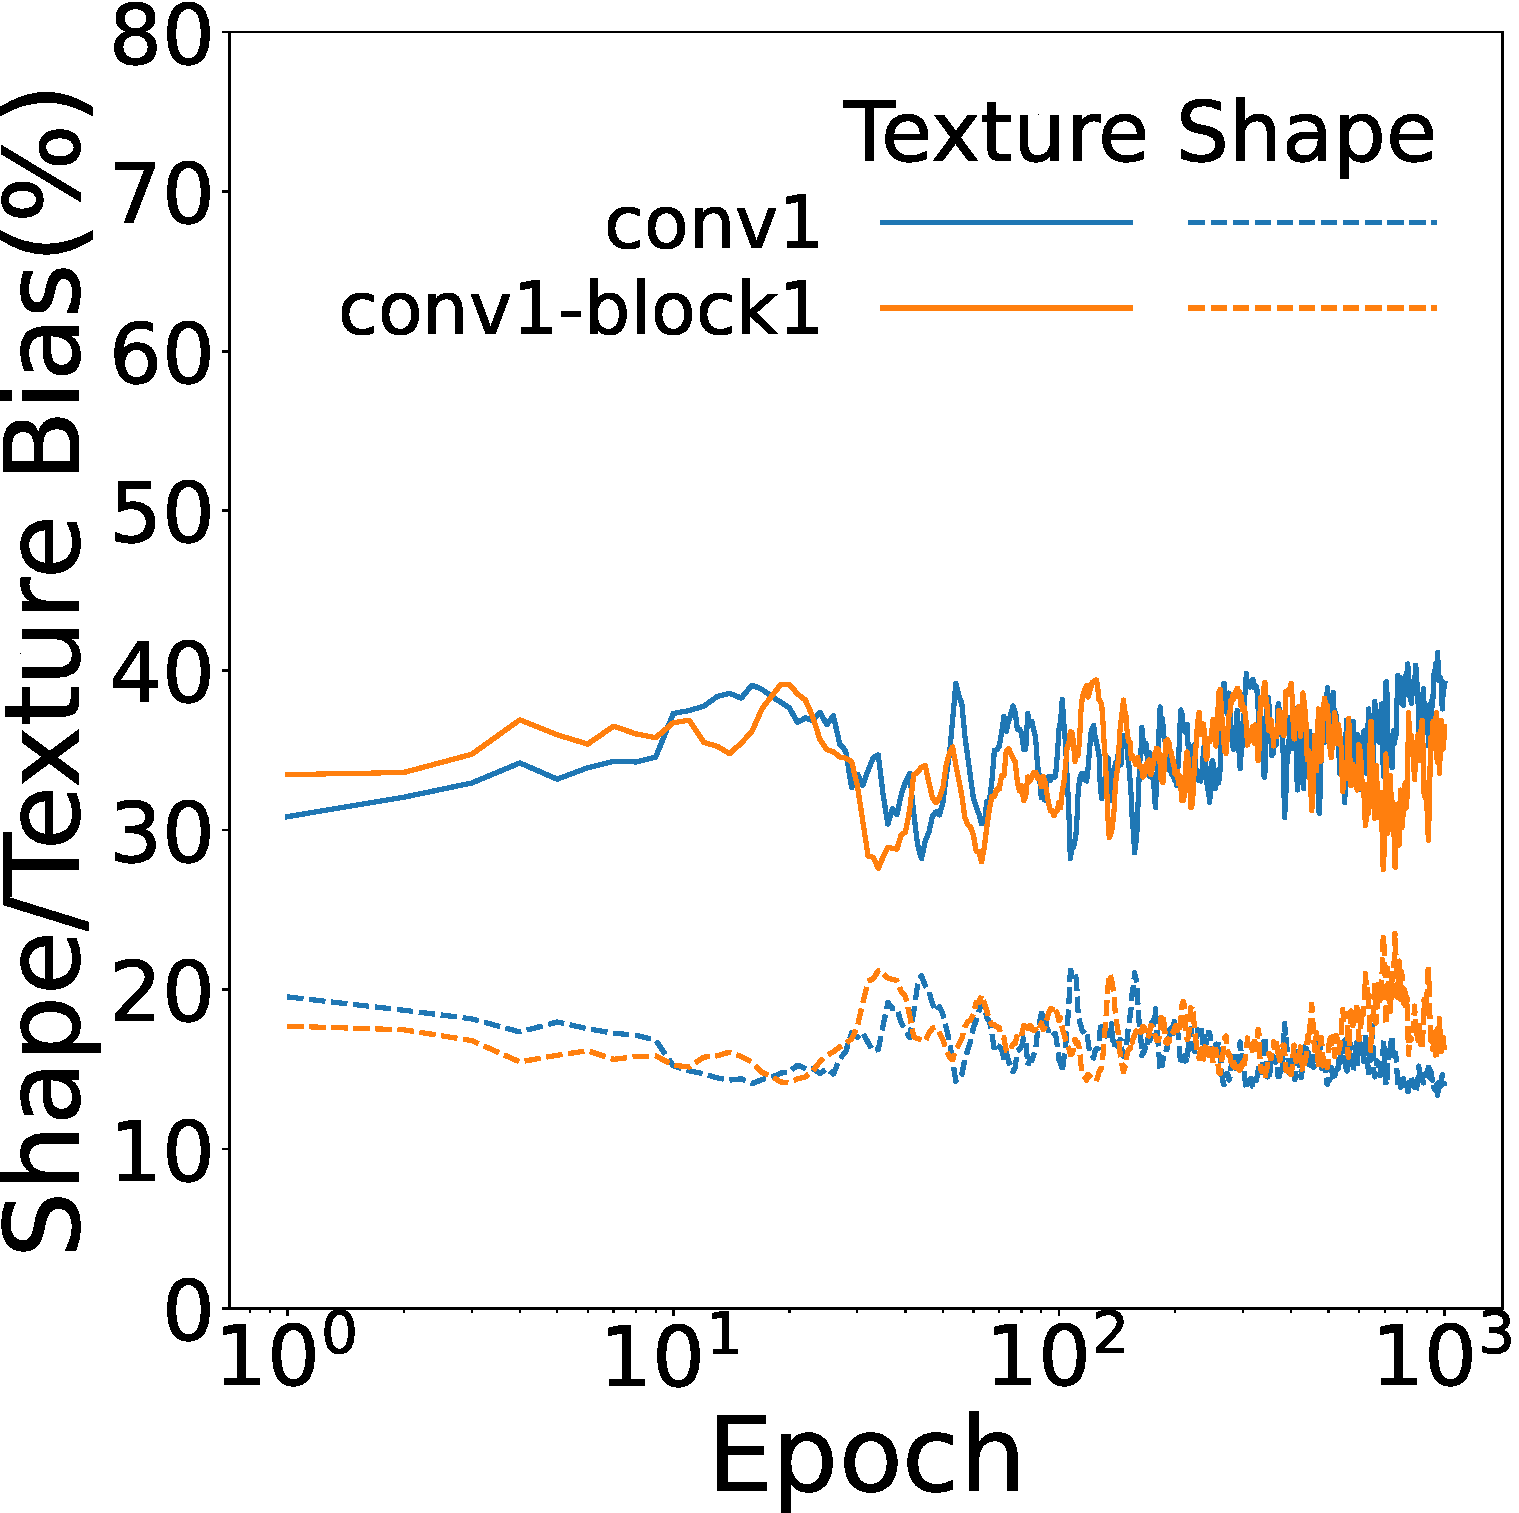
\includegraphics[keepaspectratio, width=0.45\linewidth]{fig/frozen_shallow_layer_sha_tex.pdf}
   \end{tabular}
\caption[Learning processes under shallow layer parameter freezes.]{Learning processes under shallow layer parameter freezes. Left: train/test errors Right: shape/texture bias values.}
%Learning curve graphs for double descent and shape/texture bias for different label noise. \textbf{Left}:learning curve. \textbf{Right}:model's bias shift.}
\label{fig:comp_frozen_shallow_layer}
\end{figure}
\newpage